\documentclass[11pt]{article}
\usepackage{tikz}

\makeatletter
\pgfkeys{
  /pgf/lh/.initial=30  % Default angle is 30 degrees
}

% Declare meaningful coordinate registers
\newdimen\my@N  % North (top) y coordinate
\newdimen\my@E  % East (right) x coordinate
\newdimen\my@W  % West (left) x coordinate
\newdimen\my@S  % South (bottom) y coordinate
\newdimen\my@Cx % Center x coordinate
\newdimen\my@Cy % Center y coordinate

% Other useful registers
\newdimen\my@halfwidth
\newdimen\my@halfheight
\newdimen\my@offset

% Macro to set NESW coordinates from southwest/northeast
\def\setmy@NEWSC{%
  \southwest
  \my@W=\pgf@x%
  \my@S=\pgf@y%
  \northeast
  \my@E=\pgf@x%
  \my@N=\pgf@y%
  % Calculate center
  \my@Cx=.5\my@W%
  \advance\my@Cx by.5\my@E%
  \my@Cy=.5\my@S%
  \advance\my@Cy by.5\my@N%
  % Calculate half dimensions
  \my@halfwidth=\my@E%
  \advance\my@halfwidth by-\my@W%
  \my@halfwidth=.5\my@halfwidth%
  \my@halfheight=\my@N%
  \advance\my@halfheight by-\my@S%
  \my@halfheight=.5\my@halfheight%
}

\pgfdeclareshape{lh}{
  % Inherit anchors from rectangle
  \inheritsavedanchors[from=rectangle]
  \inheritanchor[from=rectangle]{center}
  \inheritanchor[from=rectangle]{north}
  \inheritanchor[from=rectangle]{south}
  \inheritanchor[from=rectangle]{east}
  \inheritanchor[from=rectangle]{west}
  \inheritanchor[from=rectangle]{north east}
  \inheritanchor[from=rectangle]{north west}
  \inheritanchor[from=rectangle]{south east}
  \inheritanchor[from=rectangle]{south west}
  
  % Saved anchor for inner north west
  \savedanchor\innernorthwest{%
    % Get text box dimensions
    \pgf@x=.5\wd\pgfnodeparttextbox%
    \pgf@y=.5\ht\pgfnodeparttextbox%
    \advance\pgf@y by.5\dp\pgfnodeparttextbox%
    % Add inner sep
    \pgfmathsetlength\my@halfwidth{\pgfkeysvalueof{/pgf/inner xsep}}%
    \pgfmathsetlength\my@halfheight{\pgfkeysvalueof{/pgf/inner ysep}}%
    \advance\pgf@x by\my@halfwidth%
    \advance\pgf@y by\my@halfheight%
    % Check minimum dimensions
    \pgfmathsetlength\my@halfwidth{\pgfkeysvalueof{/pgf/minimum width}}%
    \pgfmathsetlength\my@halfheight{\pgfkeysvalueof{/pgf/minimum height}}%
    \ifdim\pgf@x<.5\my@halfwidth\pgf@x=.5\my@halfwidth\fi%
    \ifdim\pgf@y<.5\my@halfheight\pgf@y=.5\my@halfheight\fi%
    % Store half dimensions
    \my@halfwidth=\pgf@x%
    \my@halfheight=\pgf@y%
    % Calculate offset
    \pgfmathsetmacro{\hexangle}{\pgfkeysvalueof{/pgf/lh}}%
    \show\hexangle
    \pgfmathsetlength\my@offset{\my@halfheight*tan(\hexangle)}%
    \showthe\my@offset
    % Set final position (inner north west)
    \pgf@x=-\my@halfwidth%
    \advance\pgf@x by\my@offset%
    \pgf@y=\my@halfheight%
  }
  
  % Inner anchors - COMMENTED OUT FOR TESTING
  % \anchor{inner-north-west}{\innernorthwest}
  % \anchor{inner-north-east}{\innernorthwest\pgf@x=-\pgf@x}
  % \anchor{inner-south-west}{\innernorthwest\pgf@y=-\pgf@y}
  % \anchor{inner-south-east}{\innernorthwest\pgf@x=-\pgf@x\pgf@y=-\pgf@y}
  
  % Background path
  \backgroundpath{%
    % Get NESW coordinates
    \setmy@NEWSC
    % Get angle and calculate offset
    \pgfmathsetmacro{\hexangle}{\pgfkeysvalueof{/pgf/lh}}%
    \pgfmathsetlength\my@offset{\my@halfheight*tan(\hexangle)}%
    \showthe\my@offset
    % Draw hexagon using meaningful coordinates
    \pgfpathmoveto{\pgfpoint{\my@W}{\my@Cy}}% west vertex
    \pgfpathlineto{\pgfpoint{\my@W+\my@offset}{\my@N}}% inner NW
    \pgfpathlineto{\pgfpoint{\my@E-\my@offset}{\my@N}}% inner NE
    \pgfpathlineto{\pgfpoint{\my@E}{\my@Cy}}% east vertex
    \pgfpathlineto{\pgfpoint{\my@E-\my@offset}{\my@S}}% inner SE
    \pgfpathlineto{\pgfpoint{\my@W+\my@offset}{\my@S}}% inner SW
    \pgfpathclose%
  }
}
\makeatother

\begin{document}

% Test the lh shape with default angle (30 degrees)
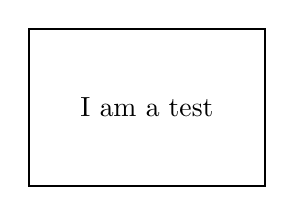
\begin{tikzpicture}
  \node[lh, draw, thick, minimum width=3cm, minimum height=2cm] (hex) at (0,0) {I am a test};
  % Debug: drop a red circle on inner north west anchor - COMMENTED OUT
  % \fill[red] (hex.inner-north-west) circle (2pt);
\end{tikzpicture}

\vspace{1cm}

% Test with different angles
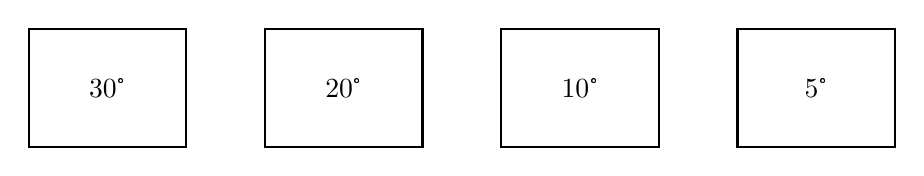
\begin{tikzpicture}
  \node[lh, draw, thick, lh=30, minimum width=2cm, minimum height=1.5cm] (hex1) at (0,0) {30°};
  % \fill[red] (hex1.inner-north-west) circle (2pt);
  
  \node[lh, draw, thick, lh=20, minimum width=2cm, minimum height=1.5cm] (hex2) at (3,0) {20°};
  % \fill[red] (hex2.inner-north-west) circle (2pt);
  
  \node[lh, draw, thick, lh=10, minimum width=2cm, minimum height=1.5cm] (hex3) at (6,0) {10°};
  % \fill[red] (hex3.inner-north-west) circle (2pt);
  
  \node[lh, draw, thick, lh=5, minimum width=2cm, minimum height=1.5cm] (hex4) at (9,0) {5°};
  % \fill[red] (hex4.inner-north-west) circle (2pt);
\end{tikzpicture}

\vspace{1cm}

% Test with different styling and show all inner anchors
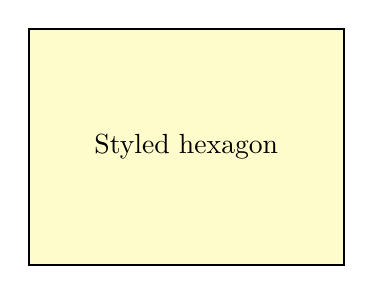
\begin{tikzpicture}
  \node[lh, draw, thick, fill=yellow!20, lh=25, minimum width=4cm, minimum height=3cm] (hex) at (0,0) {Styled hexagon};
  % Show all inner anchors - COMMENTED OUT
  % \fill[red] (hex.inner-north-west) circle (2pt) node[above left, font=\tiny] {inner NW};
  % \fill[blue] (hex.inner-north-east) circle (2pt) node[above right, font=\tiny] {inner NE};
  % \fill[green] (hex.inner-south-west) circle (2pt) node[below left, font=\tiny] {inner SW};
  % \fill[orange] (hex.inner-south-east) circle (2pt) node[below right, font=\tiny] {inner SE};
\end{tikzpicture}

\end{document}

\documentclass[11pt]{article}
\usepackage{tikz}

\makeatletter
\pgfkeys{
  /pgf/lh/.initial=30  % Default angle is 30 degrees
}

% Declare meaningful coordinate registers
\newdimen\my@N  % North (top) y coordinate
\newdimen\my@E  % East (right) x coordinate
\newdimen\my@W  % West (left) x coordinate
\newdimen\my@S  % South (bottom) y coordinate
\newdimen\my@Cx % Center x coordinate
\newdimen\my@Cy % Center y coordinate

% Other useful registers
\newdimen\my@halfwidth
\newdimen\my@halfheight
\newdimen\my@offset

% Macro to set NESW coordinates from southwest/northeast
\def\setmy@NEWSC{%
  \southwest
  \my@W=\pgf@x%
  \my@S=\pgf@y%
  \northeast
  \my@E=\pgf@x%
  \my@N=\pgf@y%
  % Calculate center
  \my@Cx=.5\my@W%
  \advance\my@Cx by.5\my@E%
  \my@Cy=.5\my@S%
  \advance\my@Cy by.5\my@N%
  % Calculate half dimensions
  \my@halfwidth=\my@E%
  \advance\my@halfwidth by-\my@W%
  \my@halfwidth=.5\my@halfwidth%
  \my@halfheight=\my@N%
  \advance\my@halfheight by-\my@S%
  \my@halfheight=.5\my@halfheight%
}

\pgfdeclareshape{lh}{
  % Inherit anchors from rectangle
  \inheritsavedanchors[from=rectangle]
  \inheritanchor[from=rectangle]{center}
  \inheritanchor[from=rectangle]{north}
  \inheritanchor[from=rectangle]{south}
  \inheritanchor[from=rectangle]{east}
  \inheritanchor[from=rectangle]{west}
  \inheritanchor[from=rectangle]{north east}
  \inheritanchor[from=rectangle]{north west}
  \inheritanchor[from=rectangle]{south east}
  \inheritanchor[from=rectangle]{south west}
  
  % Saved macro for angle
  \savedmacro\hexangle{%
    \pgfmathsetmacro{\hexangle}{\pgfkeysvalueof{/pgf/dndhexagon}}%
  }
  
  % Saved anchor for inner north west
  \savedanchor\innernorthwest{%
    % Get text box dimensions
    \pgf@x=.5\wd\pgfnodeparttextbox%
    \pgf@y=.5\ht\pgfnodeparttextbox%
    \advance\pgf@y by.5\dp\pgfnodeparttextbox%
    % Add inner sep
    \pgfmathsetlength\my@halfwidth{\pgfkeysvalueof{/pgf/inner xsep}}%
    \pgfmathsetlength\my@halfheight{\pgfkeysvalueof{/pgf/inner ysep}}%
    \advance\pgf@x by\my@halfwidth%
    \advance\pgf@y by\my@halfheight%
    % Check minimum dimensions
    \pgfmathsetlength\my@halfwidth{\pgfkeysvalueof{/pgf/minimum width}}%
    \pgfmathsetlength\my@halfheight{\pgfkeysvalueof{/pgf/minimum height}}%
    \ifdim\pgf@x<.5\my@halfwidth\pgf@x=.5\my@halfwidth\fi%
    \ifdim\pgf@y<.5\my@halfheight\pgf@y=.5\my@halfheight\fi%
    % Store half dimensions
    \my@halfwidth=\pgf@x%
    \my@halfheight=\pgf@y%
    % Calculate offset
    \pgfmathsetmacro{\hexangle}{\pgfkeysvalueof{/pgf/dndhexagon}}%
    \pgfmathsetlength\my@offset{\my@halfheight*tan(\hexangle)}%
    % Set final position (inner north west)
    \pgf@x=-\my@halfwidth%
    \advance\pgf@x by\my@offset%
    \pgf@y=\my@halfheight%
  }
  
  % Inner anchors
  \anchor{inner-north-west}{\innernorthwest}
  \anchor{inner-north-east}{\innernorthwest\pgf@x=-\pgf@x}
  \anchor{inner-south-west}{\innernorthwest\pgf@y=-\pgf@y}
  \anchor{inner-south-east}{\innernorthwest\pgf@x=-\pgf@x\pgf@y=-\pgf@y}
  
  % Background path
  \backgroundpath{%
    % Get NESW coordinates
    \setmy@NEWSC
    % Get angle and calculate offset
    \hexangle%
    \pgfmathsetlength\my@offset{\my@halfheight*tan(\hexangle)}%
    % Draw hexagon using meaningful coordinates
    \pgfpathmoveto{\pgfpoint{\my@W}{\my@Cy}}% west vertex
    \pgfpathlineto{\pgfpoint{\my@W+\my@offset}{\my@N}}% inner NW
    \pgfpathlineto{\pgfpoint{\my@E-\my@offset}{\my@N}}% inner NE
    \pgfpathlineto{\pgfpoint{\my@E}{\my@Cy}}% east vertex
    \pgfpathlineto{\pgfpoint{\my@E-\my@offset}{\my@S}}% inner SE
    \pgfpathlineto{\pgfpoint{\my@W+\my@offset}{\my@S}}% inner SW
    \pgfpathclose%
  }
}
\makeatother

\begin{document}

% Test the dndhexagon shape with default angle (30 degrees)
\begin{tikzpicture}
  \node[dndhexagon, draw, thick, minimum width=3cm, minimum height=2cm] (hex) at (0,0) {I am a test};
  % Debug: drop a red circle on inner north west anchor
  \fill[red] (hex.inner-north-west) circle (2pt);
\end{tikzpicture}

\vspace{1cm}

% Test with different angles
\begin{tikzpicture}
  \node[dndhexagon, draw, thick, dndhexagon=30, minimum width=2cm, minimum height=1.5cm] (hex1) at (0,0) {30°};
  \fill[red] (hex1.inner-north-west) circle (2pt);
  
  \node[dndhexagon, draw, thick, dndhexagon=20, minimum width=2cm, minimum height=1.5cm] (hex2) at (3,0) {20°};
  \fill[red] (hex2.inner-north-west) circle (2pt);
  
  \node[dndhexagon, draw, thick, dndhexagon=10, minimum width=2cm, minimum height=1.5cm] (hex3) at (6,0) {10°};
  \fill[red] (hex3.inner-north-west) circle (2pt);
  
  \node[dndhexagon, draw, thick, dndhexagon=5, minimum width=2cm, minimum height=1.5cm] (hex4) at (9,0) {5°};
  \fill[red] (hex4.inner-north-west) circle (2pt);
\end{tikzpicture}

\vspace{1cm}

% Test with different styling and show all inner anchors
\begin{tikzpicture}
  \node[dndhexagon, draw, thick, fill=yellow!20, dndhexagon=25, minimum width=4cm, minimum height=3cm] (hex) at (0,0) {Styled hexagon};
  % Show all inner anchors
  \fill[red] (hex.inner-north-west) circle (2pt) node[above left, font=\tiny] {inner NW};
  \fill[blue] (hex.inner-north-east) circle (2pt) node[above right, font=\tiny] {inner NE};
  \fill[green] (hex.inner-south-west) circle (2pt) node[below left, font=\tiny] {inner SW};
  \fill[orange] (hex.inner-south-east) circle (2pt) node[below right, font=\tiny] {inner SE};
\end{tikzpicture}

\end{document}

\documentclass[11pt]{article}
\usepackage{tikz}

\makeatletter
\pgfkeys{
  /pgf/dndhexagon/.initial=30  % Default angle is 30 degrees
}

% Declare meaningful coordinate registers
\newdimen\my@N  % North (top) y coordinate
\newdimen\my@E  % East (right) x coordinate
\newdimen\my@W  % West (left) x coordinate
\newdimen\my@S  % South (bottom) y coordinate
\newdimen\my@Cx % Center x coordinate
\newdimen\my@Cy % Center y coordinate

% Other useful registers
\newdimen\my@halfwidth
\newdimen\my@halfheight
\newdimen\my@offset

% Macro to set NESW coordinates from southwest/northeast
\def\setmy@NEWSC{%
  \southwest
  \my@W=\pgf@x%
  \my@S=\pgf@y%
  \northeast
  \my@E=\pgf@x%
  \my@N=\pgf@y%
  % Calculate center
  \my@Cx=.5\my@W%
  \advance\my@Cx by.5\my@E%
  \my@Cy=.5\my@S%
  \advance\my@Cy by.5\my@N%
  % Calculate half dimensions
  \my@halfwidth=\my@E%
  \advance\my@halfwidth by-\my@W%
  \my@halfwidth=.5\my@halfwidth%
  \my@halfheight=\my@N%
  \advance\my@halfheight by-\my@S%
  \my@halfheight=.5\my@halfheight%
}

\pgfdeclareshape{dndhexagon}{
  % Inherit anchors from rectangle
  \inheritsavedanchors[from=rectangle]
  \inheritanchor[from=rectangle]{center}
  \inheritanchor[from=rectangle]{north}
  \inheritanchor[from=rectangle]{south}
  \inheritanchor[from=rectangle]{east}
  \inheritanchor[from=rectangle]{west}
  \inheritanchor[from=rectangle]{north east}
  \inheritanchor[from=rectangle]{north west}
  \inheritanchor[from=rectangle]{south east}
  \inheritanchor[from=rectangle]{south west}
  
  % Saved macro for angle
  \savedmacro\hexangle{%
    \pgfmathsetmacro{\hexangle}{\pgfkeysvalueof{/pgf/dndhexagon}}%
  }
  
  % Saved anchor for inner north west
  \savedanchor\innernorthwest{%
    % Get text box dimensions
    \pgf@x=.5\wd\pgfnodeparttextbox%
    \pgf@y=.5\ht\pgfnodeparttextbox%
    \advance\pgf@y by.5\dp\pgfnodeparttextbox%
    % Add inner sep
    \pgfmathsetlength\my@halfwidth{\pgfkeysvalueof{/pgf/inner xsep}}%
    \pgfmathsetlength\my@halfheight{\pgfkeysvalueof{/pgf/inner ysep}}%
    \advance\pgf@x by\my@halfwidth%
    \advance\pgf@y by\my@halfheight%
    % Check minimum dimensions
    \pgfmathsetlength\my@halfwidth{\pgfkeysvalueof{/pgf/minimum width}}%
    \pgfmathsetlength\my@halfheight{\pgfkeysvalueof{/pgf/minimum height}}%
    \ifdim\pgf@x<.5\my@halfwidth\pgf@x=.5\my@halfwidth\fi%
    \ifdim\pgf@y<.5\my@halfheight\pgf@y=.5\my@halfheight\fi%
    % Store half dimensions
    \my@halfwidth=\pgf@x%
    \my@halfheight=\pgf@y%
    % Calculate offset
    \pgfmathsetmacro{\hexangle}{\pgfkeysvalueof{/pgf/dndhexagon}}%
    \pgfmathsetlength\my@offset{\my@halfheight*tan(\hexangle)}%
    % Set final position (inner north west)
    \pgf@x=-\my@halfwidth%
    \advance\pgf@x by\my@offset%
    \pgf@y=\my@halfheight%
  }
  
  % Inner anchors
  \anchor{inner north west}{\innernorthwest}
  \anchor{inner north east}{\innernorthwest\pgf@x=-\pgf@x}
  \anchor{inner south west}{\innernorthwest\pgf@y=-\pgf@y}
  \anchor{inner south east}{\innernorthwest\pgf@x=-\pgf@x\pgf@y=-\pgf@y}
  
  % Background path
  \backgroundpath{%
    % Get NESW coordinates
    \setmy@NEWSC
    % Get angle and calculate offset
    \hexangle%
    \pgfmathsetlength\my@offset{\my@halfheight*tan(\hexangle)}%
    % Draw hexagon using meaningful coordinates
    \pgfpathmoveto{\pgfpoint{\my@W}{\my@Cy}}% west vertex
    \pgfpathlineto{\pgfpoint{\my@W+\my@offset}{\my@N}}% inner NW
    \pgfpathlineto{\pgfpoint{\my@E-\my@offset}{\my@N}}% inner NE
    \pgfpathlineto{\pgfpoint{\my@E}{\my@Cy}}% east vertex
    \pgfpathlineto{\pgfpoint{\my@E-\my@offset}{\my@S}}% inner SE
    \pgfpathlineto{\pgfpoint{\my@W+\my@offset}{\my@S}}% inner SW
    \pgfpathclose%
  }
}
\makeatother

\begin{document}

% Test the dndhexagon shape with default angle (30 degrees)
\begin{tikzpicture}
  \node[dndhexagon, draw, thick, minimum width=3cm, minimum height=2cm] (hex) at (0,0) {I am a test};
  % Debug: drop a red circle on inner north west anchor
  \fill[red] (hex.inner north west) circle (2pt);
\end{tikzpicture}

\vspace{1cm}

% Test with different angles
\begin{tikzpicture}
  \node[dndhexagon, draw, thick, dndhexagon=30, minimum width=2cm, minimum height=1.5cm] (hex1) at (0,0) {30°};
  \fill[red] (hex1.inner north west) circle (2pt);
  
  \node[dndhexagon, draw, thick, dndhexagon=20, minimum width=2cm, minimum height=1.5cm] (hex2) at (3,0) {20°};
  \fill[red] (hex2.inner north west) circle (2pt);
  
  \node[dndhexagon, draw, thick, dndhexagon=10, minimum width=2cm, minimum height=1.5cm] (hex3) at (6,0) {10°};
  \fill[red] (hex3.inner north west) circle (2pt);
  
  \node[dndhexagon, draw, thick, dndhexagon=5, minimum width=2cm, minimum height=1.5cm] (hex4) at (9,0) {5°};
  \fill[red] (hex4.inner north west) circle (2pt);
\end{tikzpicture}

\vspace{1cm}

% Test with different styling and show all inner anchors
\begin{tikzpicture}
  \node[dndhexagon, draw, thick, fill=yellow!20, dndhexagon=25, minimum width=4cm, minimum height=3cm] (hex) at (0,0) {Styled hexagon};
  % Show all inner anchors
  \fill[red] (hex.inner north west) circle (2pt) node[above left, font=\tiny] {inner NW};
  \fill[blue] (hex.inner north east) circle (2pt) node[above right, font=\tiny] {inner NE};
  \fill[green] (hex.inner south west) circle (2pt) node[below left, font=\tiny] {inner SW};
  \fill[orange] (hex.inner south east) circle (2pt) node[below right, font=\tiny] {inner SE};
\end{tikzpicture}

\end{document}

\documentclass[11pt]{article}
\usepackage{tikz}

% Define the longhexagon shape
\makeatletter
\pgfkeys{
  /pgf/longhexagon/.initial=30  % Default angle is 30 degrees
}

% Declare our own temporary registers
\newdimen\my@xa
\newdimen\my@ya
\newdimen\my@xb
\newdimen\my@yb
\newdimen\my@xc
\newdimen\my@yc
\newdimen\my@xd
\newdimen\my@yd
\newdimen\my@xe
\newdimen\my@ye
\newdimen\my@xf
\newdimen\my@yf
\newdimen\my@xg
\newdimen\my@yg
\newdimen\my@xh
\newdimen\my@yh
\newdimen\my@halfwidth
\newdimen\my@halfheight
\newdimen\my@offset

\pgfdeclareshape{longhexagon}{%
  % Inherit anchors from rectangle
  \inheritsavedanchors[from=rectangle]
  \inheritanchor[from=rectangle]{center}
  \inheritanchor[from=rectangle]{north}
  \inheritanchor[from=rectangle]{south}
  \inheritanchor[from=rectangle]{east}
  \inheritanchor[from=rectangle]{west}
  \inheritanchor[from=rectangle]{north east}
  \inheritanchor[from=rectangle]{north west}
  \inheritanchor[from=rectangle]{south east}
  \inheritanchor[from=rectangle]{south west}
  
  % Background path
  \backgroundpath{%
    % Get corners
    \southwest
    \my@xa=\pgf@x%
    \my@ya=\pgf@y%
    \northeast
    \my@xb=\pgf@x%
    \my@yb=\pgf@y%
    % Draw a simple triangle: southwest - north - southeast - close
    \pgfpathmoveto{\pgfpoint{\my@xa}{\my@ya}}% SW
    \pgfpathlineto{\pgfpoint{0.5\my@xa+0.5\my@xb}{\my@yb}}% N (center top)
    \pgfpathlineto{\pgfpoint{\my@xb}{\my@ya}}% SE
    \pgfpathclose%
  }
}
\makeatother

\begin{document}

% First test: just the basic shape
\begin{tikzpicture}
  \node[longhexagon, draw, thick, minimum width=3cm, minimum height=2cm] (hex) at (0,0) {Basic test};
\end{tikzpicture}

\vspace{1cm}

% Second test: different angles
\begin{tikzpicture}
  \node[longhexagon, draw, thick, longhexagon=30, minimum width=2cm, minimum height=1.5cm] at (0,0) {30°};
  \node[longhexagon, draw, thick, longhexagon=20, minimum width=2cm, minimum height=1.5cm] at (3,0) {20°};
  \node[longhexagon, draw, thick, longhexagon=10, minimum width=2cm, minimum height=1.5cm] at (6,0) {10°};
  \node[longhexagon, draw, thick, longhexagon=5, minimum width=2cm, minimum height=1.5cm] at (9,0) {5°};
\end{tikzpicture}

\vspace{1cm}

% Third test: just standard anchors
\begin{tikzpicture}
  \node[longhexagon, draw, thick, fill=yellow!20, minimum width=4cm, minimum height=3cm] (hex) at (0,0) {Test anchors};
  % Test standard anchors first
  \fill[red] (hex.north) circle (2pt) node[above, font=\tiny] {N};
  \fill[blue] (hex.east) circle (2pt) node[right, font=\tiny] {E};
  \fill[green] (hex.south) circle (2pt) node[below, font=\tiny] {S};
  \fill[orange] (hex.west) circle (2pt) node[left, font=\tiny] {W};
\end{tikzpicture}

\end{document}

\documentclass[11pt]{article}
\usepackage{tikz}

% Define the longhexagon shape
\makeatletter
\pgfkeys{
  /pgf/longhexagon/.initial=30  % Default angle is 30 degrees
}

% Declare our own temporary registers
\newdimen\my@xa
\newdimen\my@ya
\newdimen\my@xb
\newdimen\my@yb
\newdimen\my@xc
\newdimen\my@yc
\newdimen\my@xd
\newdimen\my@yd
\newdimen\my@xe
\newdimen\my@ye
\newdimen\my@xf
\newdimen\my@yf
\newdimen\my@xg
\newdimen\my@yg
\newdimen\my@xh
\newdimen\my@yh
\newdimen\my@halfwidth
\newdimen\my@halfheight
\newdimen\my@offset

\pgfdeclareshape{longhexagon}{%
  % Inherit anchors from rectangle
  \inheritsavedanchors[from=rectangle]
  \inheritanchor[from=rectangle]{center}
  \inheritanchor[from=rectangle]{north}
  \inheritanchor[from=rectangle]{south}
  \inheritanchor[from=rectangle]{east}
  \inheritanchor[from=rectangle]{west}
  \inheritanchor[from=rectangle]{north east}
  \inheritanchor[from=rectangle]{north west}
  \inheritanchor[from=rectangle]{south east}
  \inheritanchor[from=rectangle]{south west}
  
  % Background path
  \backgroundpath{%
    % Get corners
    \southwest
    \my@xa=\pgf@x%
    \my@ya=\pgf@y%
    \northeast
    \my@xb=\pgf@x%
    \my@yb=\pgf@y%
    % Calculate dimensions
    \my@halfheight=\my@yb%
    \advance\my@halfheight by-\my@ya%
    \my@halfheight=.5\my@halfheight%
    % Calculate middle y
    \my@yc=\my@ya%
    \advance\my@yc by\my@halfheight%
    % Get angle and calculate offset
    \pgfmathsetmacro{\hexangle}{\pgfkeysvalueof{/pgf/longhexagon}}%
    % Debug: Check if angle is being read
    \ifdim\hexangle pt=30pt%
      % Angle is default 30
    \fi%
    % Calculate offset = halfheight * tan(angle)
    \pgfmathsetlength{\my@offset}{\my@halfheight*tan(30)}%
    % Just draw a simple hexagon for now
    \pgfpathmoveto{\pgfpoint{\my@xa}{\my@yc}}% west
%    \pgfpathlineto{\pgfpoint{\my@xa+1cm}{\my@yb}}% NW
%    \pgfpathlineto{\pgfpoint{\my@xb-1cm}{\my@yb}}% NE
    \pgfpathlineto{\pgfpoint{\my@xb}{\my@yc}}% east
%    \pgfpathlineto{\pgfpoint{\my@xb-\my@offset}{\my@ya}}% SE
    \pgfpathlineto{\pgfpoint{\my@xa+\my@offset}{\my@ya+1cm}}% SW
    \pgfpathclose%
  }
}
\makeatother

\begin{document}

% First test: just the basic shape
\begin{tikzpicture}
  \node[longhexagon, draw, thick, minimum width=3cm, minimum height=2cm] (hex) at (0,0) {Basic test};
\end{tikzpicture}

\vspace{1cm}

% Second test: different angles
\begin{tikzpicture}
  \node[longhexagon, draw, thick, longhexagon=30, minimum width=2cm, minimum height=1.5cm] at (0,0) {30°};
  \node[longhexagon, draw, thick, longhexagon=20, minimum width=2cm, minimum height=1.5cm] at (3,0) {20°};
  \node[longhexagon, draw, thick, longhexagon=10, minimum width=2cm, minimum height=1.5cm] at (6,0) {10°};
  \node[longhexagon, draw, thick, longhexagon=5, minimum width=2cm, minimum height=1.5cm] at (9,0) {5°};
\end{tikzpicture}

\vspace{1cm}

% Third test: just standard anchors
\begin{tikzpicture}
  \node[longhexagon, draw, thick, fill=yellow!20, minimum width=4cm, minimum height=3cm] (hex) at (0,0) {Test anchors};
  % Test standard anchors first
  \fill[red] (hex.north) circle (2pt) node[above, font=\tiny] {Nx};
  \fill[blue] (hex.east) circle (2pt) node[right, font=\tiny] {E};
  \fill[green] (hex.south) circle (2pt) node[below, font=\tiny] {S};
  \fill[orange] (hex.west) circle (2pt) node[left, font=\tiny] {W};
\end{tikzpicture}

\end{document}

\documentclass[11pt]{article}
\usepackage{tikz}

% Define the longhexagon shape
\makeatletter
\pgfkeys{
  /pgf/longhexagon/.initial=30  % Default angle is 30 degrees
}

% Declare our own temporary registers
\newdimen\my@xa
\newdimen\my@ya
\newdimen\my@xb
\newdimen\my@yb
\newdimen\my@xc
\newdimen\my@yc
\newdimen\my@xd
\newdimen\my@yd
\newdimen\my@xe
\newdimen\my@ye
\newdimen\my@xf
\newdimen\my@yf
\newdimen\my@xg
\newdimen\my@yg
\newdimen\my@xh
\newdimen\my@yh
\newdimen\my@halfwidth
\newdimen\my@halfheight
\newdimen\my@offset

\pgfdeclareshape{longhexagon}{%
  % Inherit anchors from rectangle
  \inheritsavedanchors[from=rectangle]
  \inheritanchor[from=rectangle]{center}
  \inheritanchor[from=rectangle]{north}
  \inheritanchor[from=rectangle]{south}
  \inheritanchor[from=rectangle]{east}
  \inheritanchor[from=rectangle]{west}
  \inheritanchor[from=rectangle]{north east}
  \inheritanchor[from=rectangle]{north west}
  \inheritanchor[from=rectangle]{south east}
  \inheritanchor[from=rectangle]{south west}
  
  % Background path
  \backgroundpath{%
    % Get corners
    \southwest
    \my@xa=\pgf@x%
    \my@ya=\pgf@y%
    \northeast
    \my@xb=\pgf@x%
    \my@yb=\pgf@y%
    % Calculate dimensions
    \my@halfheight=\my@yb%
    \advance\my@halfheight by-\my@ya%
    \my@halfheight=.5\my@halfheight%
    % Get angle and calculate offset
    \pgfmathsetmacro{\hexangle}{\pgfkeysvalueof{/pgf/longhexagon}}%
    \pgfmathsetlength\my@offset{\my@halfheight*tan(\hexangle)}%
    % Calculate vertices
    % v1: west
    \my@xc=\my@xa%
    \my@yc=\my@ya%
    \advance\my@yc by\my@halfheight%
    % v2: inner north west
    \my@xd=\my@xa%
    \advance\my@xd by\my@offset%
    \my@yd=\my@yb%
    % v3: inner north east
    \my@xe=\my@xb%
    \advance\my@xe by-\my@offset%
    \my@ye=\my@yb%
    % v4: east
    \my@xf=\my@xb%
    \my@yf=\my@ya%
    \advance\my@yf by\my@halfheight%
    % v5: inner south east
    \my@xg=\my@xb%
    \advance\my@xg by-\my@offset%
    \my@yg=\my@ya%
    % v6: inner south west
    \my@xh=\my@xa%
    \advance\my@xh by\my@offset%
    \my@yh=\my@ya%
    % Draw path
    \pgfpathmoveto{\pgfpoint{\my@xc}{\my@yc}}%
    \pgfpathlineto{\pgfpoint{\my@xd}{\my@yd}}%
    \pgfpathlineto{\pgfpoint{\my@xe}{\my@ye}}%
    \pgfpathlineto{\pgfpoint{\my@xf}{\my@yf}}%
    \pgfpathlineto{\pgfpoint{\my@xg}{\my@yg}}%
    \pgfpathlineto{\pgfpoint{\my@xh}{\my@yh}}%
    \pgfpathclose%
  }
}
\makeatother

\begin{document}

% First test: just the basic shape
\begin{tikzpicture}
  \node[longhexagon, draw, thick, minimum width=3cm, minimum height=2cm] (hex) at (0,0) {Basic test};
\end{tikzpicture}

\vspace{1cm}

% Second test: different angles
\begin{tikzpicture}
  \node[longhexagon, draw, thick, longhexagon=30, minimum width=2cm, minimum height=1.5cm] at (0,0) {30°};
  \node[longhexagon, draw, thick, longhexagon=20, minimum width=2cm, minimum height=1.5cm] at (3,0) {20°};
  \node[longhexagon, draw, thick, longhexagon=10, minimum width=2cm, minimum height=1.5cm] at (6,0) {10°};
  \node[longhexagon, draw, thick, longhexagon=5, minimum width=2cm, minimum height=1.5cm] at (9,0) {5°};
\end{tikzpicture}

\vspace{1cm}

% Third test: just standard anchors
\begin{tikzpicture}
  \node[longhexagon, draw, thick, fill=yellow!20, minimum width=4cm, minimum height=3cm] (hex) at (0,0) {Test anchors};
  % Test standard anchors first
  \fill[red] (hex.north) circle (2pt) node[above, font=\tiny] {N};
  \fill[blue] (hex.east) circle (2pt) node[right, font=\tiny] {E};
  \fill[green] (hex.south) circle (2pt) node[below, font=\tiny] {S};
  \fill[orange] (hex.west) circle (2pt) node[left, font=\tiny] {W};
\end{tikzpicture}

\end{document}


\documentclass[11pt]{article}
\usepackage{tikz}
\usetikzlibrary{calc}

% Define the longhexagon shape
\makeatletter
\pgfkeys{
  /pgf/longhexagon/.initial=30  % Default angle is 30 degrees
}

% Declare our own temporary registers
\newdimen\my@xa
\newdimen\my@ya
\newdimen\my@xb
\newdimen\my@yb
\newdimen\my@xc
\newdimen\my@yc
\newdimen\my@xd
\newdimen\my@yd
\newdimen\my@xe
\newdimen\my@ye
\newdimen\my@xf
\newdimen\my@yf
\newdimen\my@xg
\newdimen\my@yg
\newdimen\my@xh
\newdimen\my@yh
\newdimen\my@halfwidth
\newdimen\my@halfheight
\newdimen\my@offset

\pgfdeclareshape{longhexagon}{%
  % Inherit anchors from rectangle
  \inheritsavedanchors[from=rectangle]
  \inheritanchor[from=rectangle]{center}
  \inheritanchor[from=rectangle]{north}
  \inheritanchor[from=rectangle]{south}
  \inheritanchor[from=rectangle]{east}
  \inheritanchor[from=rectangle]{west}
  \inheritanchor[from=rectangle]{north east}
  \inheritanchor[from=rectangle]{north west}
  \inheritanchor[from=rectangle]{south east}
  \inheritanchor[from=rectangle]{south west}
  
  % Saved macro for angle
  \savedmacro\hexangle{%
    \pgfmathsetmacro{\hexangle}{\pgfkeysvalueof{/pgf/longhexagon}}%
  }
  
  % Saved anchor for inner north west
  \savedanchor\innernorthwest{%
    % Get text box dimensions
    \my@halfwidth=.5\wd\pgfnodeparttextbox%
    \my@halfheight=.5\ht\pgfnodeparttextbox%
    \advance\my@halfheight by.5\dp\pgfnodeparttextbox%
    % Add inner sep
    \pgfmathsetlength\my@xa{\pgfkeysvalueof{/pgf/inner xsep}}%
    \pgfmathsetlength\my@ya{\pgfkeysvalueof{/pgf/inner ysep}}%
    \advance\my@halfwidth by\my@xa%
    \advance\my@halfheight by\my@ya%
    % Check minimum dimensions
    \pgfmathsetlength\my@xb{\pgfkeysvalueof{/pgf/minimum width}}%
    \pgfmathsetlength\my@yb{\pgfkeysvalueof{/pgf/minimum height}}%
    \my@xb=.5\my@xb%
    \my@yb=.5\my@yb%
    \ifdim\my@halfwidth<\my@xb\my@halfwidth=\my@xb\fi%
    \ifdim\my@halfheight<\my@yb\my@halfheight=\my@yb\fi%
    % Calculate offset
    \pgfmathsetmacro{\hexangle}{\pgfkeysvalueof{/pgf/longhexagon}}%
    \pgfmathsetlength\my@offset{\my@halfheight*tan(\hexangle)}%
    % Set final position
    \pgf@x=-\my@halfwidth%
    \advance\pgf@x by\my@offset%
    \pgf@y=\my@halfheight%
  }
  
  % Inner anchors
  \anchor{inner north west}{\innernorthwest}
  \anchor{inner north east}{\innernorthwest\pgf@x=-\pgf@x}
  \anchor{inner south west}{\innernorthwest\pgf@y=-\pgf@y}
  \anchor{inner south east}{\innernorthwest\pgf@x=-\pgf@x\pgf@y=-\pgf@y}
  
  % Background path
  \backgroundpath{%
    % Get corners
    \southwest
    \my@xa=\pgf@x%
    \my@ya=\pgf@y%
    \northeast
    \my@xb=\pgf@x%
    \my@yb=\pgf@y%
    % Calculate dimensions
    \my@halfwidth=\my@xb%
    \advance\my@halfwidth by-\my@xa%
    \my@halfwidth=.5\my@halfwidth%
    \my@halfheight=\my@yb%
    \advance\my@halfheight by-\my@ya%
    \my@halfheight=.5\my@halfheight%
    % Get angle and calculate offset
    \hexangle%
    \pgfmathsetlength\my@offset{\my@halfheight*tan(\hexangle)}%
    % Calculate vertices
    % v1: west
    \my@xc=\my@xa%
    \my@yc=\my@ya%
    \advance\my@yc by\my@halfheight%
    % v2: inner north west
    \my@xd=\my@xa%
    \advance\my@xd by\my@offset%
    \my@yd=\my@yb%
    % v3: inner north east
    \my@xe=\my@xb%
    \advance\my@xe by-\my@offset%
    \my@ye=\my@yb%
    % v4: east
    \my@xf=\my@xb%
    \my@yf=\my@ya%
    \advance\my@yf by\my@halfheight%
    % v5: inner south east
    \my@xg=\my@xb%
    \advance\my@xg by-\my@offset%
    \my@yg=\my@ya%
    % v6: inner south west
    \my@xh=\my@xa%
    \advance\my@xh by\my@offset%
    \my@yh=\my@ya%
    % Draw path
    \pgfpathmoveto{\pgfpoint{\my@xc}{\my@yc}}%
    \pgfpathlineto{\pgfpoint{\my@xd}{\my@yd}}%
    \pgfpathlineto{\pgfpoint{\my@xe}{\my@ye}}%
    \pgfpathlineto{\pgfpoint{\my@xf}{\my@yf}}%
    \pgfpathlineto{\pgfpoint{\my@xg}{\my@yg}}%
    \pgfpathlineto{\pgfpoint{\my@xh}{\my@yh}}%
    \pgfpathclose%
  }
}
\makeatother

\begin{document}

% Test the longhexagon shape with default angle (30 degrees)
\begin{tikzpicture}
  \node[longhexagon, draw, thick, minimum width=3cm, minimum height=2cm] (hex) at (0,0) {I am a test};
  % Debug: drop a red circle on inner north west anchor
  \fill[red] (hex.inner north west) circle (2pt);
\end{tikzpicture}

\vspace{1cm}

% Test with different angles
\begin{tikzpicture}
  \node[longhexagon, draw, thick, longhexagon=30, minimum width=2cm, minimum height=1.5cm] (hex1) at (0,0) {30°};
  \fill[red] (hex1.inner north west) circle (2pt);
  
  \node[longhexagon, draw, thick, longhexagon=20, minimum width=2cm, minimum height=1.5cm] (hex2) at (3,0) {20°};
  \fill[red] (hex2.inner north west) circle (2pt);
  
  \node[longhexagon, draw, thick, longhexagon=10, minimum width=2cm, minimum height=1.5cm] (hex3) at (6,0) {10°};
  \fill[red] (hex3.inner north west) circle (2pt);
  
  \node[longhexagon, draw, thick, longhexagon=5, minimum width=2cm, minimum height=1.5cm] (hex4) at (9,0) {5°};
  \fill[red] (hex4.inner north west) circle (2pt);
\end{tikzpicture}

\vspace{1cm}

% Test with different styling and show all inner anchors
\begin{tikzpicture}
  \node[longhexagon, draw, thick, fill=yellow!20, longhexagon=25, minimum width=4cm, minimum height=3cm] (hex) at (0,0) {Styled hexagon};
  % Show all inner anchors
  \fill[red] (hex.inner north west) circle (2pt) node[above left, font=\tiny] {inner NW};
  \fill[blue] (hex.inner north east) circle (2pt) node[above right, font=\tiny] {inner NE};
  \fill[green] (hex.inner south west) circle (2pt) node[below left, font=\tiny] {inner SW};
  \fill[orange] (hex.inner south east) circle (2pt) node[below right, font=\tiny] {inner SE};
\end{tikzpicture}

\end{document}

%%\documentclass[11pt]{article}
%%\usepackage{tikz}
%%\usetikzlibrary{calc}
%%
%%% Define the longhexagon shape
%%\makeatletter
%%\pgfkeys{
%%  /pgf/longhexagon/.initial=30  % Default angle is 30 degrees
%%}
%%
%%\pgfdeclareshape{longhexagon}{
%%  % Inherit anchors from rectangle
%%  \inheritsavedanchors[from=rectangle]
%%  \inheritanchor[from=rectangle]{center}
%%  \inheritanchor[from=rectangle]{north}
%%  \inheritanchor[from=rectangle]{south}
%%  \inheritanchor[from=rectangle]{east}
%%  \inheritanchor[from=rectangle]{west}
%%  \inheritanchor[from=rectangle]{north east}
%%  \inheritanchor[from=rectangle]{north west}
%%  \inheritanchor[from=rectangle]{south east}
%%  \inheritanchor[from=rectangle]{south west}
%%  
%%  % Saved macro for angle (computed once)
%%  \savedmacro\hexangle{%
%%    \pgfmathsetmacro{\hexangle}{\pgfkeysvalueof{/pgf/longhexagon}}%
%%    \pgfmathsetmacro{\hexangle}{\pgfkeysvalueof{/pgf/longhexagon}}%
%%  }
%%  
%%  % Saved anchor for inner north west
%%  \savedanchor\innernorthwest{%
%%    \pgf@x=.5\wd\pgfnodeparttextbox%
%%    \pgf@y=.5\ht\pgfnodeparttextbox%
%%    \advance\pgf@y by.5\dp\pgfnodeparttextbox%
%%    \pgfmathsetlength\pgf@xb{\pgfkeysvalueof{/pgf/inner xsep}}%
%%    \pgfmathsetlength\pgf@yb{\pgfkeysvalueof{/pgf/inner ysep}}%
%%    \advance\pgf@x by\pgf@xb%
%%    \advance\pgf@y by\pgf@yb%
%%    \pgfmathsetlength\pgf@xc{\pgfkeysvalueof{/pgf/minimum width}}%
%%    \pgfmathsetlength\pgf@yc{\pgfkeysvalueof{/pgf/minimum height}}%
%%    \ifdim\pgf@x<.5\pgf@xc\pgf@x=.5\pgf@xc\fi%
%%    \ifdim\pgf@y<.5\pgf@yc\pgf@y=.5\pgf@yc\fi%
%%    % Now we have half dimensions, compute inner north west
%%    \pgfmathsetmacro{\hexangle}{\pgfkeysvalueof{/pgf/longhexagon}}%
%%    \pgfmathsetlength\pgf@xa{\pgf@y*tan(\hexangle)}% offset = halfheight * tan(angle)
%%    \pgf@x=-\pgf@x%  % west side (negative half-width)
%%    \advance\pgf@x by\pgf@xa%  % adjust inward by angle offset
%%    % pgf@y already contains positive half-height, which is north
%%  }
%%  
%%  % Inner north west anchor
%%  \anchor{inner north west}{\innernorthwest}
%%  
%%  % Inner north east anchor
%%  \anchor{inner north east}{%
%%    \innernorthwest%
%%    \pgf@x=-\pgf@x%
%%  }
%%  
%%  % Inner south west anchor
%%  \anchor{inner south west}{%
%%    \innernorthwest%
%%    \pgf@y=-\pgf@y%
%%  }
%%  
%%  % Inner south east anchor
%%  \anchor{inner south east}{%
%%    \innernorthwest%
%%    \pgf@x=-\pgf@x%
%%    \pgf@y=-\pgf@y%
%%  }
%%  
%%  % Background path (defines the shape outline)
%%  \backgroundpath{%
%%    % Get the corners
%%    \southwest\pgf@xa=\pgf@x\pgf@ya=\pgf@y%
%%    \northeast\pgf@xb=\pgf@x\pgf@yb=\pgf@y%
%%    % Get the saved angle
%%    \hexangle%
%%    % Calculate vertices
%%    % West point
%%    \pgf@xc=\pgf@xa%
%%    \pgf@yc=.5\pgf@ya%
%%    \advance\pgf@yc by.5\pgf@yb%
%%    % Height for offset calculation
%%    \pgf@ytemp=\pgf@yb%
%%    \advance\pgf@ytemp by-\pgf@ya%
%%    \pgf@ytemp=.5\pgf@ytemp%
%%    \pgfmathsetlength\pgf@xtemp{\pgf@ytemp*tan(\hexangle)}%
%%    % Inner north west
%%    \pgf@xd=\pgf@xa%
%%    \advance\pgf@xd by\pgf@xtemp%
%%    \pgf@yd=\pgf@yb%
%%    % Inner north east  
%%    \pgf@xe=\pgf@xb%
%%    \advance\pgf@xe by-\pgf@xtemp%
%%    \pgf@ye=\pgf@yb%
%%    % East point
%%    \pgf@xf=\pgf@xb%
%%    \pgf@yf=\pgf@yc%
%%    % Inner south east
%%    \pgf@xg=\pgf@xb%
%%    \advance\pgf@xg by-\pgf@xtemp%
%%    \pgf@yg=\pgf@ya%
%%    % Inner south west
%%    \pgf@xh=\pgf@xa%
%%    \advance\pgf@xh by\pgf@xtemp%
%%    \pgf@yh=\pgf@ya%
%%    % Draw the path
%%    \pgfpathmoveto{\pgfpoint{\pgf@xc}{\pgf@yc}}%
%%    \pgfpathlineto{\pgfpoint{\pgf@xd}{\pgf@yd}}%
%%    \pgfpathlineto{\pgfpoint{\pgf@xe}{\pgf@ye}}%
%%    \pgfpathlineto{\pgfpoint{\pgf@xf}{\pgf@yf}}%
%%    \pgfpathlineto{\pgfpoint{\pgf@xg}{\pgf@yg}}%
%%    \pgfpathlineto{\pgfpoint{\pgf@xh}{\pgf@yh}}%
%%    \pgfpathclose%
%%  }
%%}
%%\makeatother
%%
%%\begin{document}
%%
%%% Test the longhexagon shape with default angle (30 degrees)
%%\begin{tikzpicture}
%%  \node[longhexagon, draw, thick, minimum width=3cm, minimum height=2cm] (hex) at (0,0) {I am a test};
%%  % Debug: drop a red circle on inner north west anchor
%%  \fill[red] (hex.inner north west) circle (2pt);
%%\end{tikzpicture}
%%
%%\vspace{1cm}
%%
%%% Test with different angles
%%\begin{tikzpicture}
%%  \node[longhexagon, draw, thick, longhexagon=30, minimum width=2cm, minimum height=1.5cm] (hex1) at (0,0) {30°};
%%  \fill[red] (hex1.inner north west) circle (2pt);
%%  
%%  \node[longhexagon, draw, thick, longhexagon=20, minimum width=2cm, minimum height=1.5cm] (hex2) at (3,0) {20°};
%%  \fill[red] (hex2.inner north west) circle (2pt);
%%  
%%  \node[longhexagon, draw, thick, longhexagon=10, minimum width=2cm, minimum height=1.5cm] (hex3) at (6,0) {10°};
%%  \fill[red] (hex3.inner north west) circle (2pt);
%%  
%%  \node[longhexagon, draw, thick, longhexagon=5, minimum width=2cm, minimum height=1.5cm] (hex4) at (9,0) {5°};
%%  \fill[red] (hex4.inner north west) circle (2pt);
%%\end{tikzpicture}
%%
%%\vspace{1cm}
%%
%%% Test with different styling and show all inner anchors
%%\begin{tikzpicture}
%%  \node[longhexagon, draw, thick, fill=yellow!20, longhexagon=25, minimum width=4cm, minimum height=3cm] (hex) at (0,0) {Styled hexagon};
%%  % Show all inner anchors
%%  \fill[red] (hex.inner north west) circle (2pt) node[above left, font=\tiny] {inner NW};
%%  \fill[blue] (hex.inner north east) circle (2pt) node[above right, font=\tiny] {inner NE};
%%  \fill[green] (hex.inner south west) circle (2pt) node[below left, font=\tiny] {inner SW};
%%  \fill[orange] (hex.inner south east) circle (2pt) node[below right, font=\tiny] {inner SE};
%%  
%%  % Also show standard anchors for comparison
%%  \draw[gray] (hex.north west) circle (1pt) node[above left, font=\tiny, gray] {NW};
%%  \draw[gray] (hex.north east) circle (1pt) node[above right, font=\tiny, gray] {NE};
%%\end{tikzpicture}
%%
%%\end{document}
%%
%%\documentclass[11pt]{article}
%%\usepackage{tikz}
%%\usetikzlibrary{calc}
%%
%%% Define the longhexagon shape
%%\makeatletter
%%\pgfkeys{
%%  /pgf/longhexagon/.initial=30  % Default angle is 30 degrees
%%}
%%
%%\pgfdeclareshape{longhexagon}{
%%  % Inherit anchors from rectangle
%%  \inheritsavedanchors[from=rectangle]
%%  \inheritanchor[from=rectangle]{center}
%%  \inheritanchor[from=rectangle]{north}
%%  \inheritanchor[from=rectangle]{south}
%%  \inheritanchor[from=rectangle]{east}
%%  \inheritanchor[from=rectangle]{west}
%%  \inheritanchor[from=rectangle]{north east}
%%  \inheritanchor[from=rectangle]{north west}
%%  \inheritanchor[from=rectangle]{south east}
%%  \inheritanchor[from=rectangle]{south west}
%%  
%%  % Saved macro for angle (computed once)
%%  \savedmacro\hexangle{%
%%    \pgfmathsetmacro{\hexangle}{\pgfkeysvalueof{/pgf/longhexagon}}%
%%  }
%%  
%%  % Saved anchor for inner north west
%%  \savedanchor\innernorthwest{%
%%    \pgf@x=.5\wd\pgfnodeparttextbox%
%%    \pgf@y=.5\ht\pgfnodeparttextbox%
%%    \advance\pgf@y by.5\dp\pgfnodeparttextbox%
%%    \pgfmathsetlength\pgf@xb{\pgfkeysvalueof{/pgf/inner xsep}}%
%%    \pgfmathsetlength\pgf@yb{\pgfkeysvalueof{/pgf/inner ysep}}%
%%    \advance\pgf@x by\pgf@xb%
%%    \advance\pgf@y by\pgf@yb%
%%    \pgfmathsetlength\pgf@xc{\pgfkeysvalueof{/pgf/minimum width}}%
%%    \pgfmathsetlength\pgf@yc{\pgfkeysvalueof{/pgf/minimum height}}%
%%    \ifdim\pgf@x<.5\pgf@xc\pgf@x=.5\pgf@xc\fi%
%%    \ifdim\pgf@y<.5\pgf@yc\pgf@y=.5\pgf@yc\fi%
%%    % Now we have half dimensions, compute inner north west
%%    \pgfmathsetmacro{\hexangle}{\pgfkeysvalueof{/pgf/longhexagon}}%
%%    \pgfmathsetlength\pgf@xa{\pgf@y*tan(\hexangle)}%
%%    \pgf@y=-\pgf@y%  % Make it relative to center
%%    \pgf@x=-\pgf@x%  % west side
%%    \advance\pgf@x by\pgf@xa%  % adjust by angle offset
%%    \pgf@y=-\pgf@y%  % north side
%%  }
%%  
%%  % Inner north west anchor
%%  \anchor{inner north west}{\innernorthwest}
%%  
%%  % Inner north east anchor
%%  \anchor{inner north east}{%
%%    \innernorthwest%
%%    \pgf@x=-\pgf@x%
%%  }
%%  
%%  % Inner south west anchor
%%  \anchor{inner south west}{%
%%    \innernorthwest%
%%    \pgf@y=-\pgf@y%
%%  }
%%  
%%  % Inner south east anchor
%%  \anchor{inner south east}{%
%%    \innernorthwest%
%%    \pgf@x=-\pgf@x%
%%    \pgf@y=-\pgf@y%
%%  }
%%  
%%  % Background path (defines the shape outline)
%%  \backgroundpath{%
%%    % Get the corners
%%    \southwest\pgf@xa=\pgf@x\pgf@ya=\pgf@y%
%%    \northeast\pgf@xb=\pgf@x\pgf@yb=\pgf@y%
%%    % Get the saved angle
%%    \hexangle%
%%    % Calculate vertices
%%    % West point
%%    \pgf@xc=\pgf@xa%
%%    \pgf@yc=.5\pgf@ya%
%%    \advance\pgf@yc by.5\pgf@yb%
%%    % Height for offset calculation
%%    \pgf@ytemp=\pgf@yb%
%%    \advance\pgf@ytemp by-\pgf@ya%
%%    \pgf@ytemp=.5\pgf@ytemp%
%%    \pgfmathsetlength\pgf@xtemp{\pgf@ytemp*tan(\hexangle)}%
%%    % Inner north west
%%    \pgf@xd=\pgf@xa%
%%    \advance\pgf@xd by\pgf@xtemp%
%%    \pgf@yd=\pgf@yb%
%%    % Inner north east  
%%    \pgf@xe=\pgf@xb%
%%    \advance\pgf@xe by-\pgf@xtemp%
%%    \pgf@ye=\pgf@yb%
%%    % East point
%%    \pgf@xf=\pgf@xb%
%%    \pgf@yf=\pgf@yc%
%%    % Inner south east
%%    \pgf@xg=\pgf@xb%
%%    \advance\pgf@xg by-\pgf@xtemp%
%%    \pgf@yg=\pgf@ya%
%%    % Inner south west
%%    \pgf@xh=\pgf@xa%
%%    \advance\pgf@xh by\pgf@xtemp%
%%    \pgf@yh=\pgf@ya%
%%    % Draw the path
%%    \pgfpathmoveto{\pgfpoint{\pgf@xc}{\pgf@yc}}%
%%    \pgfpathlineto{\pgfpoint{\pgf@xd}{\pgf@yd}}%
%%    \pgfpathlineto{\pgfpoint{\pgf@xe}{\pgf@ye}}%
%%    \pgfpathlineto{\pgfpoint{\pgf@xf}{\pgf@yf}}%
%%    \pgfpathlineto{\pgfpoint{\pgf@xg}{\pgf@yg}}%
%%    \pgfpathlineto{\pgfpoint{\pgf@xh}{\pgf@yh}}%
%%    \pgfpathclose%
%%  }
%%}
%%\makeatother
%%
%%\begin{document}
%%
%%% Test the longhexagon shape with default angle (30 degrees)
%%\begin{tikzpicture}
%%  \node[longhexagon, draw, thick, minimum width=3cm, minimum height=2cm] (hex) at (0,0) {I am a test};
%%  % Debug: drop a red circle on inner north west anchor
%%  \fill[red] (hex.inner north west) circle (2pt);
%%\end{tikzpicture}
%%
%%\vspace{1cm}
%%
%%% Test with different angles
%%\begin{tikzpicture}
%%  \node[longhexagon, draw, thick, longhexagon=30, minimum width=2cm, minimum height=1.5cm] (hex1) at (0,0) {30°};
%%  \fill[red] (hex1.inner north west) circle (2pt);
%%  
%%  \node[longhexagon, draw, thick, longhexagon=20, minimum width=2cm, minimum height=1.5cm] (hex2) at (3,0) {20°};
%%  \fill[red] (hex2.inner north west) circle (2pt);
%%  
%%  \node[longhexagon, draw, thick, longhexagon=10, minimum width=2cm, minimum height=1.5cm] (hex3) at (6,0) {10°};
%%  \fill[red] (hex3.inner north west) circle (2pt);
%%  
%%  \node[longhexagon, draw, thick, longhexagon=5, minimum width=2cm, minimum height=1.5cm] (hex4) at (9,0) {5°};
%%  \fill[red] (hex4.inner north west) circle (2pt);
%%\end{tikzpicture}
%%
%%\vspace{1cm}
%%
%%% Test with different styling and show all inner anchors
%%\begin{tikzpicture}
%%  \node[longhexagon, draw, thick, fill=yellow!20, longhexagon=25, minimum width=4cm, minimum height=3cm] (hex) at (0,0) {Styled hexagon};
%%  % Show all inner anchors
%%  \fill[red] (hex.inner north west) circle (2pt) node[above left, font=\tiny] {inner NW};
%%  \fill[blue] (hex.inner north east) circle (2pt) node[above right, font=\tiny] {inner NE};
%%  \fill[green] (hex.inner south west) circle (2pt) node[below left, font=\tiny] {inner SW};
%%  \fill[orange] (hex.inner south east) circle (2pt) node[below right, font=\tiny] {inner SE};
%%  
%%  % Also show standard anchors for comparison
%%  \draw[gray] (hex.north west) circle (1pt) node[above left, font=\tiny, gray] {NW};
%%  \draw[gray] (hex.north east) circle (1pt) node[above right, font=\tiny, gray] {NE};
%%\end{tikzpicture}
%%
%%\end{document}
%%
%%\documentclass[11pt]{article}
%%\usepackage{tikz}
%%\usetikzlibrary{calc}
%%
%%% Define the longhexagon shape
%%\makeatletter
%%\pgfkeys{
%%  /pgf/longhexagon/.initial=30  % Default angle is 30 degrees
%%}
%%
%%% Declare our own temporary registers
%%\newdimen\my@xa
%%\newdimen\my@ya
%%\newdimen\my@xb
%%\newdimen\my@yb
%%\newdimen\my@xc
%%\newdimen\my@yc
%%\newdimen\my@xd
%%\newdimen\my@yd
%%\newdimen\my@xe
%%\newdimen\my@ye
%%\newdimen\my@xf
%%\newdimen\my@yf
%%\newdimen\my@xg
%%\newdimen\my@yg
%%\newdimen\my@xh
%%\newdimen\my@yh
%%
%%\pgfdeclareshape{longhexagon}{
%%  % Inherit anchors from rectangle
%%  \inheritsavedanchors[from=rectangle]
%%  \inheritanchor[from=rectangle]{center}
%%  \inheritanchor[from=rectangle]{north}
%%  \inheritanchor[from=rectangle]{south}
%%  \inheritanchor[from=rectangle]{east}
%%  \inheritanchor[from=rectangle]{west}
%%  \inheritanchor[from=rectangle]{north east}
%%  \inheritanchor[from=rectangle]{north west}
%%  \inheritanchor[from=rectangle]{south east}
%%  \inheritanchor[from=rectangle]{south west}
%%  
%%  % Define inner north west anchor
%%  \anchor{inner north west}{%
%%    \southwest \my@xa=\pgf@x \my@ya=\pgf@y
%%    \northeast \my@xb=\pgf@x \my@yb=\pgf@y
%%    \pgfmathsetmacro{\hexangle}{\pgfkeysvalueof{/pgf/longhexagon}}%
%%    \pgfpointlineattime{0.5}{\pgfpoint{\my@xa}{\my@ya}}{\pgfpoint{\my@xa}{\my@yb}}%
%%    \my@xc=\pgf@x \my@yc=\pgf@y
%%    \pgfpointadd{\pgfpoint{\my@xc}{\my@yc}}{\pgfpointpolar{90-\hexangle}{1cm}}%
%%    \my@xd=\pgf@x \my@yd=\pgf@y
%%    \pgfpointintersectionoflines{\pgfpoint{\my@xc}{\my@yc}}{\pgfpoint{\my@xd}{\my@yd}}{\pgfpoint{\my@xa}{\my@yb}}{\pgfpoint{\my@xb}{\my@yb}}%
%%  }
%%  
%%  % Define inner north east anchor
%%  \anchor{inner north east}{%
%%    \southwest \my@xa=\pgf@x \my@ya=\pgf@y
%%    \northeast \my@xb=\pgf@x \my@yb=\pgf@y
%%    \pgfmathsetmacro{\hexangle}{\pgfkeysvalueof{/pgf/longhexagon}}%
%%    \pgfpointlineattime{0.5}{\pgfpoint{\my@xb}{\my@ya}}{\pgfpoint{\my@xb}{\my@yb}}%
%%    \my@xc=\pgf@x \my@yc=\pgf@y
%%    \pgfpointadd{\pgfpoint{\my@xc}{\my@yc}}{\pgfpointpolar{90+\hexangle}{1cm}}%
%%    \my@xd=\pgf@x \my@yd=\pgf@y
%%    \pgfpointintersectionoflines{\pgfpoint{\my@xc}{\my@yc}}{\pgfpoint{\my@xd}{\my@yd}}{\pgfpoint{\my@xa}{\my@yb}}{\pgfpoint{\my@xb}{\my@yb}}%
%%  }
%%  
%%  % Define inner south west anchor
%%  \anchor{inner south west}{%
%%    \southwest \my@xa=\pgf@x \my@ya=\pgf@y
%%    \northeast \my@xb=\pgf@x \my@yb=\pgf@y
%%    \pgfmathsetmacro{\hexangle}{\pgfkeysvalueof{/pgf/longhexagon}}%
%%    \pgfpointlineattime{0.5}{\pgfpoint{\my@xa}{\my@ya}}{\pgfpoint{\my@xa}{\my@yb}}%
%%    \my@xc=\pgf@x \my@yc=\pgf@y
%%    \pgfpointadd{\pgfpoint{\my@xc}{\my@yc}}{\pgfpointpolar{270+\hexangle}{1cm}}%
%%    \my@xd=\pgf@x \my@yd=\pgf@y
%%    \pgfpointintersectionoflines{\pgfpoint{\my@xc}{\my@yc}}{\pgfpoint{\my@xd}{\my@yd}}{\pgfpoint{\my@xa}{\my@ya}}{\pgfpoint{\my@xb}{\my@ya}}%
%%  }
%%  
%%  % Define inner south east anchor
%%  \anchor{inner south east}{%
%%    \southwest \my@xa=\pgf@x \my@ya=\pgf@y
%%    \northeast \my@xb=\pgf@x \my@yb=\pgf@y
%%    \pgfmathsetmacro{\hexangle}{\pgfkeysvalueof{/pgf/longhexagon}}%
%%    \pgfpointlineattime{0.5}{\pgfpoint{\my@xb}{\my@ya}}{\pgfpoint{\my@xb}{\my@yb}}%
%%    \my@xc=\pgf@x \my@yc=\pgf@y
%%    \pgfpointadd{\pgfpoint{\my@xc}{\my@yc}}{\pgfpointpolar{270-\hexangle}{1cm}}%
%%    \my@xd=\pgf@x \my@yd=\pgf@y
%%    \pgfpointintersectionoflines{\pgfpoint{\my@xc}{\my@yc}}{\pgfpoint{\my@xd}{\my@yd}}{\pgfpoint{\my@xa}{\my@ya}}{\pgfpoint{\my@xb}{\my@ya}}%
%%  }
%%  
%%  % Background path (defines the shape outline)
%%  \backgroundpath{%
%%    % Get the corners and store in our registers
%%    \southwest
%%    \my@xa=\pgf@x  % left edge
%%    \my@ya=\pgf@y  % bottom edge
%%    \northeast
%%    \my@xb=\pgf@x  % right edge
%%    \my@yb=\pgf@y  % top edge
%%    %
%%    % Get angle
%%    \pgfmathsetmacro{\hexangle}{\pgfkeysvalueof{/pgf/longhexagon}}%
%%    %
%%    % Calculate all six vertices
%%    %
%%    % v1: west (middle of left edge)
%%    \pgfpointlineattime{0.5}{\pgfpoint{\my@xa}{\my@ya}}{\pgfpoint{\my@xa}{\my@yb}}%
%%    \my@xc=\pgf@x  % Store west x
%%    \my@yc=\pgf@y  % Store west y
%%    %
%%    % v2: inner north west
%%    \pgfpointadd{\pgfpoint{\my@xc}{\my@yc}}{\pgfpointpolar{90-\hexangle}{1cm}}%
%%    \my@xd=\pgf@x
%%    \my@yd=\pgf@y
%%    \pgfpointintersectionoflines{\pgfpoint{\my@xc}{\my@yc}}{\pgfpoint{\my@xd}{\my@yd}}{\pgfpoint{\my@xa}{\my@yb}}{\pgfpoint{\my@xb}{\my@yb}}%
%%    \my@xd=\pgf@x
%%    \my@yd=\pgf@y
%%    %
%%    % v3: inner north east - first find east point
%%    \pgfpointlineattime{0.5}{\pgfpoint{\my@xb}{\my@ya}}{\pgfpoint{\my@xb}{\my@yb}}%
%%    \my@xe=\pgf@x
%%    \my@ye=\pgf@y
%%    \pgfpointadd{\pgfpoint{\my@xe}{\my@ye}}{\pgfpointpolar{90+\hexangle}{1cm}}%
%%    \my@xf=\pgf@x
%%    \my@yf=\pgf@y
%%    \pgfpointintersectionoflines{\pgfpoint{\my@xe}{\my@ye}}{\pgfpoint{\my@xf}{\my@yf}}{\pgfpoint{\my@xa}{\my@yb}}{\pgfpoint{\my@xb}{\my@yb}}%
%%    \my@xf=\pgf@x
%%    \my@yf=\pgf@y
%%    %
%%    % v4: east already stored in my@xe, my@ye
%%    %
%%    % v5: inner south east
%%    \pgfpointadd{\pgfpoint{\my@xe}{\my@ye}}{\pgfpointpolar{270-\hexangle}{1cm}}%
%%    \my@xg=\pgf@x
%%    \my@yg=\pgf@y
%%    \pgfpointintersectionoflines{\pgfpoint{\my@xe}{\my@ye}}{\pgfpoint{\my@xg}{\my@yg}}{\pgfpoint{\my@xa}{\my@ya}}{\pgfpoint{\my@xb}{\my@ya}}%
%%    \my@xg=\pgf@x
%%    \my@yg=\pgf@y
%%    %
%%    % v6: inner south west
%%    \pgfpointadd{\pgfpoint{\my@xc}{\my@yc}}{\pgfpointpolar{270+\hexangle}{1cm}}%
%%    \my@xh=\pgf@x
%%    \my@yh=\pgf@y
%%    \pgfpointintersectionoflines{\pgfpoint{\my@xc}{\my@yc}}{\pgfpoint{\my@xh}{\my@yh}}{\pgfpoint{\my@xa}{\my@ya}}{\pgfpoint{\my@xb}{\my@ya}}%
%%    \my@xh=\pgf@x
%%    \my@yh=\pgf@y
%%    %
%%    % Now draw the hexagon using our stored values
%%    \pgfpathmoveto{\pgfpoint{\my@xc}{\my@yc}}%
%%    \pgfpathlineto{\pgfpoint{\my@xd}{\my@yd}}%
%%    \pgfpathlineto{\pgfpoint{\my@xf}{\my@yf}}%
%%    \pgfpathlineto{\pgfpoint{\my@xe}{\my@ye}}%
%%    \pgfpathlineto{\pgfpoint{\my@xg}{\my@yg}}%
%%    \pgfpathlineto{\pgfpoint{\my@xh}{\my@yh}}%
%%    \pgfpathclose
%%  }
%%}
%%\makeatother
%%
%%\begin{document}
%%
%%% Test the longhexagon shape with default angle (30 degrees)
%%\begin{tikzpicture}
%%  \node[longhexagon, draw, thick, minimum width=3cm, minimum height=2cm] (hex) at (0,0) {I am a test};
%%  % Debug: drop a red circle on inner north west anchor
%%  \fill[red] (hex.inner north west) circle (2pt);
%%\end{tikzpicture}
%%
%%\vspace{1cm}
%%
%%% Test with different angles
%%\begin{tikzpicture}
%%  \node[longhexagon, draw, thick, longhexagon=30, minimum width=2cm, minimum height=1.5cm] (hex1) at (0,0) {30°};
%%  \fill[red] (hex1.inner north west) circle (2pt);
%%  
%%  \node[longhexagon, draw, thick, longhexagon=20, minimum width=2cm, minimum height=1.5cm] (hex2) at (3,0) {20°};
%%  \fill[red] (hex2.inner north west) circle (2pt);
%%  
%%  \node[longhexagon, draw, thick, longhexagon=10, minimum width=2cm, minimum height=1.5cm] (hex3) at (6,0) {10°};
%%  \fill[red] (hex3.inner north west) circle (2pt);
%%  
%%  \node[longhexagon, draw, thick, longhexagon=5, minimum width=2cm, minimum height=1.5cm] (hex4) at (9,0) {5°};
%%  \fill[red] (hex4.inner north west) circle (2pt);
%%\end{tikzpicture}
%%
%%\vspace{1cm}
%%
%%% Test with different styling and show all inner anchors
%%\begin{tikzpicture}
%%  \node[longhexagon, draw, thick, fill=yellow!20, longhexagon=25, minimum width=4cm, minimum height=3cm] (hex) at (0,0) {Styled hexagon};
%%  % Show all inner anchors
%%  \fill[red] (hex.inner north west) circle (2pt) node[above left, font=\tiny] {inner NW};
%%  \fill[blue] (hex.inner north east) circle (2pt) node[above right, font=\tiny] {inner NE};
%%  \fill[green] (hex.inner south west) circle (2pt) node[below left, font=\tiny] {inner SW};
%%  \fill[orange] (hex.inner south east) circle (2pt) node[below right, font=\tiny] {inner SE};
%%\end{tikzpicture}
%%
%%\end{document}
%%
%%\documentclass[11pt]{article}
%%\usepackage{tikz}
%%\usetikzlibrary{calc}
%%
%%% Define the longhexagon shape
%%\makeatletter
%%\pgfkeys{
%%  /pgf/longhexagon/.initial=30  % Default angle is 30 degrees
%%}
%%
%%% Declare our own temporary registers
%%\newdimen\my@xa
%%\newdimen\my@ya
%%\newdimen\my@xb
%%\newdimen\my@yb
%%\newdimen\my@xc
%%\newdimen\my@yc
%%\newdimen\my@xd
%%\newdimen\my@yd
%%\newdimen\my@xe
%%\newdimen\my@ye
%%\newdimen\my@xf
%%\newdimen\my@yf
%%\newdimen\my@xg
%%\newdimen\my@yg
%%\newdimen\my@xh
%%\newdimen\my@yh
%%
%%\pgfdeclareshape{longhexagon}{
%%  % Inherit anchors from rectangle
%%  \inheritsavedanchors[from=rectangle]
%%  \inheritanchor[from=rectangle]{center}
%%  \inheritanchor[from=rectangle]{north}
%%  \inheritanchor[from=rectangle]{south}
%%  \inheritanchor[from=rectangle]{east}
%%  \inheritanchor[from=rectangle]{west}
%%  \inheritanchor[from=rectangle]{north east}
%%  \inheritanchor[from=rectangle]{north west}
%%  \inheritanchor[from=rectangle]{south east}
%%  \inheritanchor[from=rectangle]{south west}
%%  
%%  % Define inner north west anchor
%%  \anchor{inner north west}{
%%    % Get bounding box
%%    \southwest
%%    \my@xa=\pgf@x  % left edge
%%    \my@ya=\pgf@y  % bottom edge
%%    \northeast
%%    \my@xb=\pgf@x  % right edge
%%    \my@yb=\pgf@y  % top edge
%%    
%%    % Get angle
%%    \pgfmathsetmacro{\hexangle}{\pgfkeysvalueof{/pgf/longhexagon}}
%%    
%%    % West point (middle of left edge)
%%    \pgfpointlineattime{0.5}{\pgfpoint{\my@xa}{\my@ya}}{\pgfpoint{\my@xa}{\my@yb}}
%%    \my@xc=\pgf@x
%%    \my@yc=\pgf@y
%%    
%%    % Point along the angled line from west (using polar)
%%    \pgfpointadd{\pgfpoint{\my@xc}{\my@yc}}{\pgfpointpolar{90-\hexangle}{1cm}}
%%    \my@xd=\pgf@x
%%    \my@yd=\pgf@y
%%    
%%    % Find intersection with top edge
%%    \pgfpointintersectionoflines
%%      {\pgfpoint{\my@xc}{\my@yc}}{\pgfpoint{\my@xd}{\my@yd}}
%%      {\pgfpoint{\my@xa}{\my@yb}}{\pgfpoint{\my@xb}{\my@yb}}
%%  }
%%  
%%  % Define inner north east anchor
%%  \anchor{inner north east}{
%%    % Get bounding box
%%    \southwest
%%    \my@xa=\pgf@x  % left edge
%%    \my@ya=\pgf@y  % bottom edge
%%    \northeast
%%    \my@xb=\pgf@x  % right edge
%%    \my@yb=\pgf@y  % top edge
%%    
%%    % Get angle
%%    \pgfmathsetmacro{\hexangle}{\pgfkeysvalueof{/pgf/longhexagon}}
%%    
%%    % East point (middle of right edge)
%%    \pgfpointlineattime{0.5}{\pgfpoint{\my@xb}{\my@ya}}{\pgfpoint{\my@xb}{\my@yb}}
%%    \my@xc=\pgf@x
%%    \my@yc=\pgf@y
%%    
%%    % Point along the angled line from east (using polar)
%%    \pgfpointadd{\pgfpoint{\my@xc}{\my@yc}}{\pgfpointpolar{90+\hexangle}{1cm}}
%%    \my@xd=\pgf@x
%%    \my@yd=\pgf@y
%%    
%%    % Find intersection with top edge
%%    \pgfpointintersectionoflines
%%      {\pgfpoint{\my@xc}{\my@yc}}{\pgfpoint{\my@xd}{\my@yd}}
%%      {\pgfpoint{\my@xa}{\my@yb}}{\pgfpoint{\my@xb}{\my@yb}}
%%  }
%%  
%%  % Define inner south west anchor
%%  \anchor{inner south west}{
%%    % Get bounding box
%%    \southwest
%%    \my@xa=\pgf@x  % left edge
%%    \my@ya=\pgf@y  % bottom edge
%%    \northeast
%%    \my@xb=\pgf@x  % right edge
%%    \my@yb=\pgf@y  % top edge
%%    
%%    % Get angle
%%    \pgfmathsetmacro{\hexangle}{\pgfkeysvalueof{/pgf/longhexagon}}
%%    
%%    % West point (middle of left edge)
%%    \pgfpointlineattime{0.5}{\pgfpoint{\my@xa}{\my@ya}}{\pgfpoint{\my@xa}{\my@yb}}
%%    \my@xc=\pgf@x
%%    \my@yc=\pgf@y
%%    
%%    % Point along the angled line from west (using polar)
%%    \pgfpointadd{\pgfpoint{\my@xc}{\my@yc}}{\pgfpointpolar{270+\hexangle}{1cm}}
%%    \my@xd=\pgf@x
%%    \my@yd=\pgf@y
%%    
%%    % Find intersection with bottom edge
%%    \pgfpointintersectionoflines
%%      {\pgfpoint{\my@xc}{\my@yc}}{\pgfpoint{\my@xd}{\my@yd}}
%%      {\pgfpoint{\my@xa}{\my@ya}}{\pgfpoint{\my@xb}{\my@ya}}
%%  }
%%  
%%  % Define inner south east anchor
%%  \anchor{inner south east}{
%%    % Get bounding box
%%    \southwest
%%    \my@xa=\pgf@x  % left edge
%%    \my@ya=\pgf@y  % bottom edge
%%    \northeast
%%    \my@xb=\pgf@x  % right edge
%%    \my@yb=\pgf@y  % top edge
%%    
%%    % Get angle
%%    \pgfmathsetmacro{\hexangle}{\pgfkeysvalueof{/pgf/longhexagon}}
%%    
%%    % East point (middle of right edge)
%%    \pgfpointlineattime{0.5}{\pgfpoint{\my@xb}{\my@ya}}{\pgfpoint{\my@xb}{\my@yb}}
%%    \my@xc=\pgf@x
%%    \my@yc=\pgf@y
%%    
%%    % Point along the angled line from east (using polar)
%%    \pgfpointadd{\pgfpoint{\my@xc}{\my@yc}}{\pgfpointpolar{270-\hexangle}{1cm}}
%%    \my@xd=\pgf@x
%%    \my@yd=\pgf@y
%%    
%%    % Find intersection with bottom edge
%%    \pgfpointintersectionoflines
%%      {\pgfpoint{\my@xc}{\my@yc}}{\pgfpoint{\my@xd}{\my@yd}}
%%      {\pgfpoint{\my@xa}{\my@ya}}{\pgfpoint{\my@xb}{\my@ya}}
%%  }
%%  
%%  % Background path (defines the shape outline)
%%  \backgroundpath{
%%    % Get the corners and store in our registers
%%    \southwest
%%    \my@xa=\pgf@x  % left edge
%%    \my@ya=\pgf@y  % bottom edge
%%    \northeast
%%    \my@xb=\pgf@x  % right edge
%%    \my@yb=\pgf@y  % top edge
%%    
%%    % Get angle
%%    \pgfmathsetmacro{\hexangle}{\pgfkeysvalueof{/pgf/longhexagon}}
%%    
%%    % Calculate all six vertices
%%    
%%    % v1: west (middle of left edge)
%%    \pgfpointlineattime{0.5}{\pgfpoint{\my@xa}{\my@ya}}{\pgfpoint{\my@xa}{\my@yb}}
%%    \my@xc=\pgf@x  % Store west x
%%    \my@yc=\pgf@y  % Store west y
%%    
%%    % v2: inner north west
%%    % First create a point along the angled line
%%    \pgfpointadd{\pgfpoint{\my@xc}{\my@yc}}{\pgfpointpolar{90-\hexangle}{1cm}}
%%    \my@xd=\pgf@x  % Store temp point x
%%    \my@yd=\pgf@y  % Store temp point y
%%    % Find intersection
%%    \pgfpointintersectionoflines
%%      {\pgfpoint{\my@xc}{\my@yc}}{\pgfpoint{\my@xd}{\my@yd}}
%%      {\pgfpoint{\my@xa}{\my@yb}}{\pgfpoint{\my@xb}{\my@yb}}
%%    \my@xd=\pgf@x  % Store inner north west x
%%    \my@yd=\pgf@y  % Store inner north west y
%%    
%%    % v3: inner north east
%%    % First find east point
%%    \pgfpointlineattime{0.5}{\pgfpoint{\my@xb}{\my@ya}}{\pgfpoint{\my@xb}{\my@yb}}
%%    \my@xe=\pgf@x  % Store east x
%%    \my@ye=\pgf@y  % Store east y
%%    % Create point along angled line
%%    \pgfpointadd{\pgfpoint{\my@xe}{\my@ye}}{\pgfpointpolar{90+\hexangle}{1cm}}
%%    \my@xf=\pgf@x  % Store temp point x
%%    \my@yf=\pgf@y  % Store temp point y
%%    % Find intersection
%%    \pgfpointintersectionoflines
%%      {\pgfpoint{\my@xe}{\my@ye}}{\pgfpoint{\my@xf}{\my@yf}}
%%      {\pgfpoint{\my@xa}{\my@yb}}{\pgfpoint{\my@xb}{\my@yb}}
%%    \my@xf=\pgf@x  % Store inner north east x
%%    \my@yf=\pgf@y  % Store inner north east y
%%    
%%    % v4: east (already stored in my@xe, my@ye)
%%    
%%    % v5: inner south east
%%    \pgfpointadd{\pgfpoint{\my@xe}{\my@ye}}{\pgfpointpolar{270-\hexangle}{1cm}}
%%    \my@xg=\pgf@x  % Store temp point x
%%    \my@yg=\pgf@y  % Store temp point y
%%    \pgfpointintersectionoflines
%%      {\pgfpoint{\my@xe}{\my@ye}}{\pgfpoint{\my@xg}{\my@yg}}
%%      {\pgfpoint{\my@xa}{\my@ya}}{\pgfpoint{\my@xb}{\my@ya}}
%%    \my@xg=\pgf@x  % Store inner south east x
%%    \my@yg=\pgf@y  % Store inner south east y
%%    
%%    % v6: inner south west
%%    \pgfpointadd{\pgfpoint{\my@xc}{\my@yc}}{\pgfpointpolar{270+\hexangle}{1cm}}
%%    \my@xh=\pgf@x  % Store temp point x
%%    \my@yh=\pgf@y  % Store temp point y
%%    \pgfpointintersectionoflines
%%      {\pgfpoint{\my@xc}{\my@yc}}{\pgfpoint{\my@xh}{\my@yh}}
%%      {\pgfpoint{\my@xa}{\my@ya}}{\pgfpoint{\my@xb}{\my@ya}}
%%    \my@xh=\pgf@x  % Store inner south west x
%%    \my@yh=\pgf@y  % Store inner south west y
%%    
%%    % Now draw the hexagon using our stored values
%%    \pgfpathmoveto{\pgfpoint{\my@xc}{\my@yc}}  % v1 (west)
%%    \pgfpathlineto{\pgfpoint{\my@xd}{\my@yd}}  % v2 (inner north west)
%%    \pgfpathlineto{\pgfpoint{\my@xf}{\my@yf}}  % v3 (inner north east)
%%    \pgfpathlineto{\pgfpoint{\my@xe}{\my@ye}}  % v4 (east)
%%    \pgfpathlineto{\pgfpoint{\my@xg}{\my@yg}}  % v5 (inner south east)
%%    \pgfpathlineto{\pgfpoint{\my@xh}{\my@yh}}  % v6 (inner south west)
%%    \pgfpathclose
%%  }
%%}
%%\makeatother
%%
%%\begin{document}
%%
%%% Test the longhexagon shape with default angle (30 degrees)
%%\begin{tikzpicture}
%%  \node[longhexagon, draw, thick, minimum width=3cm, minimum height=2cm] (hex) at (0,0) {I am a test};
%%  % Debug: drop a red circle on inner north west anchor
%%  \fill[red] (hex.inner north west) circle (2pt);
%%\end{tikzpicture}
%%
%%\vspace{1cm}
%%
%%% Test with different angles
%%\begin{tikzpicture}
%%  \node[longhexagon, draw, thick, longhexagon=30, minimum width=2cm, minimum height=1.5cm] (hex1) at (0,0) {30°};
%%  \fill[red] (hex1.inner north west) circle (2pt);
%%  
%%  \node[longhexagon, draw, thick, longhexagon=20, minimum width=2cm, minimum height=1.5cm] (hex2) at (3,0) {20°};
%%  \fill[red] (hex2.inner north west) circle (2pt);
%%  
%%  \node[longhexagon, draw, thick, longhexagon=10, minimum width=2cm, minimum height=1.5cm] (hex3) at (6,0) {10°};
%%  \fill[red] (hex3.inner north west) circle (2pt);
%%  
%%  \node[longhexagon, draw, thick, longhexagon=5, minimum width=2cm, minimum height=1.5cm] (hex4) at (9,0) {5°};
%%  \fill[red] (hex4.inner north west) circle (2pt);
%%\end{tikzpicture}
%%
%%\vspace{1cm}
%%
%%% Test with different styling and show all inner anchors
%%\begin{tikzpicture}
%%  \node[longhexagon, draw, thick, fill=yellow!20, longhexagon=25, minimum width=4cm, minimum height=3cm] (hex) at (0,0) {Styled hexagon};
%%  % Show all inner anchors
%%  \fill[red] (hex.inner north west) circle (2pt) node[above left, font=\tiny] {inner NW};
%%  \fill[blue] (hex.inner north east) circle (2pt) node[above right, font=\tiny] {inner NE};
%%  \fill[green] (hex.inner south west) circle (2pt) node[below left, font=\tiny] {inner SW};
%%  \fill[orange] (hex.inner south east) circle (2pt) node[below right, font=\tiny] {inner SE};
%%\end{tikzpicture}
%%
%%\end{document}
%%
%%\documentclass[11pt]{article}
%%\usepackage{tikz}
%%\usetikzlibrary{calc}
%%
%%% Define the longhexagon shape
%%\makeatletter
%%\pgfkeys{
%%  /pgf/longhexagon/.initial=30  % Default angle is 30 degrees
%%}
%%
%%% Declare our own temporary registers
%%\newdimen\my@xa
%%\newdimen\my@ya
%%\newdimen\my@xb
%%\newdimen\my@yb
%%\newdimen\my@xc
%%\newdimen\my@yc
%%\newdimen\my@xd
%%\newdimen\my@yd
%%\newdimen\my@xe
%%\newdimen\my@ye
%%\newdimen\my@xf
%%\newdimen\my@yf
%%\newdimen\my@xg
%%\newdimen\my@yg
%%\newdimen\my@xh
%%\newdimen\my@yh
%%
%%\pgfdeclareshape{longhexagon}{
%%  % Inherit anchors from rectangle
%%  \inheritsavedanchors[from=rectangle]
%%  \inheritanchor[from=rectangle]{center}
%%  \inheritanchor[from=rectangle]{north}
%%  \inheritanchor[from=rectangle]{south}
%%  \inheritanchor[from=rectangle]{east}
%%  \inheritanchor[from=rectangle]{west}
%%  \inheritanchor[from=rectangle]{north east}
%%  \inheritanchor[from=rectangle]{north west}
%%  \inheritanchor[from=rectangle]{south east}
%%  \inheritanchor[from=rectangle]{south west}
%%  
%%  % Define inner north west anchor
%%  \anchor{inner north west}{
%%    % Get bounding box
%%    \southwest
%%    \my@xa=\pgf@x  % left edge
%%    \my@ya=\pgf@y  % bottom edge
%%    \northeast
%%    \my@xb=\pgf@x  % right edge
%%    \my@yb=\pgf@y  % top edge
%%    
%%    % Get angle
%%    \pgfmathsetmacro{\hexangle}{\pgfkeysvalueof{/pgf/longhexagon}}
%%    
%%    % West point (middle of left edge)
%%    \pgfpointlineattime{0.5}{\pgfpoint{\my@xa}{\my@ya}}{\pgfpoint{\my@xa}{\my@yb}}
%%    \my@xc=\pgf@x
%%    \my@yc=\pgf@y
%%    
%%    % Point along the angled line from west (using polar)
%%    \pgfpointadd{\pgfpoint{\my@xc}{\my@yc}}{\pgfpointpolar{90-\hexangle}{1cm}}
%%    \my@xd=\pgf@x
%%    \my@yd=\pgf@y
%%    
%%    % Find intersection with top edge
%%    \pgfpointintersectionoflines
%%      {\pgfpoint{\my@xc}{\my@yc}}{\pgfpoint{\my@xd}{\my@yd}}
%%      {\pgfpoint{\my@xa}{\my@yb}}{\pgfpoint{\my@xb}{\my@yb}}
%%  }
%%  
%%  % Define inner north east anchor
%%  \anchor{inner north east}{
%%    % Get bounding box
%%    \southwest
%%    \my@xa=\pgf@x  % left edge
%%    \my@ya=\pgf@y  % bottom edge
%%    \northeast
%%    \my@xb=\pgf@x  % right edge
%%    \my@yb=\pgf@y  % top edge
%%    
%%    % Get angle
%%    \pgfmathsetmacro{\hexangle}{\pgfkeysvalueof{/pgf/longhexagon}}
%%    
%%    % East point (middle of right edge)
%%    \pgfpointlineattime{0.5}{\pgfpoint{\my@xb}{\my@ya}}{\pgfpoint{\my@xb}{\my@yb}}
%%    \my@xc=\pgf@x
%%    \my@yc=\pgf@y
%%    
%%    % Point along the angled line from east (using polar)
%%    \pgfpointadd{\pgfpoint{\my@xc}{\my@yc}}{\pgfpointpolar{90+\hexangle}{1cm}}
%%    \my@xd=\pgf@x
%%    \my@yd=\pgf@y
%%    
%%    % Find intersection with top edge
%%    \pgfpointintersectionoflines
%%      {\pgfpoint{\my@xc}{\my@yc}}{\pgfpoint{\my@xd}{\my@yd}}
%%      {\pgfpoint{\my@xa}{\my@yb}}{\pgfpoint{\my@xb}{\my@yb}}
%%  }
%%  
%%  % Define inner south west anchor
%%  \anchor{inner south west}{
%%    % Get bounding box
%%    \southwest
%%    \my@xa=\pgf@x  % left edge
%%    \my@ya=\pgf@y  % bottom edge
%%    \northeast
%%    \my@xb=\pgf@x  % right edge
%%    \my@yb=\pgf@y  % top edge
%%    
%%    % Get angle
%%    \pgfmathsetmacro{\hexangle}{\pgfkeysvalueof{/pgf/longhexagon}}
%%    
%%    % West point (middle of left edge)
%%    \pgfpointlineattime{0.5}{\pgfpoint{\my@xa}{\my@ya}}{\pgfpoint{\my@xa}{\my@yb}}
%%    \my@xc=\pgf@x
%%    \my@yc=\pgf@y
%%    
%%    % Point along the angled line from west (using polar)
%%    \pgfpointadd{\pgfpoint{\my@xc}{\my@yc}}{\pgfpointpolar{270+\hexangle}{1cm}}
%%    \my@xd=\pgf@x
%%    \my@yd=\pgf@y
%%    
%%    % Find intersection with bottom edge
%%    \pgfpointintersectionoflines
%%      {\pgfpoint{\my@xc}{\my@yc}}{\pgfpoint{\my@xd}{\my@yd}}
%%      {\pgfpoint{\my@xa}{\my@ya}}{\pgfpoint{\my@xb}{\my@ya}}
%%  }
%%  
%%  % Define inner south east anchor
%%  \anchor{inner south east}{
%%    % Get bounding box
%%    \southwest
%%    \my@xa=\pgf@x  % left edge
%%    \my@ya=\pgf@y  % bottom edge
%%    \northeast
%%    \my@xb=\pgf@x  % right edge
%%    \my@yb=\pgf@y  % top edge
%%    
%%    % Get angle
%%    \pgfmathsetmacro{\hexangle}{\pgfkeysvalueof{/pgf/longhexagon}}
%%    
%%    % East point (middle of right edge)
%%    \pgfpointlineattime{0.5}{\pgfpoint{\my@xb}{\my@ya}}{\pgfpoint{\my@xb}{\my@yb}}
%%    \my@xc=\pgf@x
%%    \my@yc=\pgf@y
%%    
%%    % Point along the angled line from east (using polar)
%%    \pgfpointadd{\pgfpoint{\my@xc}{\my@yc}}{\pgfpointpolar{270-\hexangle}{1cm}}
%%    \my@xd=\pgf@x
%%    \my@yd=\pgf@y
%%    
%%    % Find intersection with bottom edge
%%    \pgfpointintersectionoflines
%%      {\pgfpoint{\my@xc}{\my@yc}}{\pgfpoint{\my@xd}{\my@yd}}
%%      {\pgfpoint{\my@xa}{\my@ya}}{\pgfpoint{\my@xb}{\my@ya}}
%%  }
%%  
%%  % Background path (defines the shape outline)
%%  \backgroundpath{
%%    % Get the corners and store in our registers
%%    \southwest
%%    \my@xa=\pgf@x  % left edge
%%    \my@ya=\pgf@y  % bottom edge
%%    \northeast
%%    \my@xb=\pgf@x  % right edge
%%    \my@yb=\pgf@y  % top edge
%%    
%%    % Get angle
%%    \pgfmathsetmacro{\hexangle}{\pgfkeysvalueof{/pgf/longhexagon}}
%%    
%%    % Calculate all six vertices
%%    
%%    % v1: west (middle of left edge)
%%    \pgfpointlineattime{0.5}{\pgfpoint{\my@xa}{\my@ya}}{\pgfpoint{\my@xa}{\my@yb}}
%%    \my@xc=\pgf@x  % Store west x
%%    \my@yc=\pgf@y  % Store west y
%%    
%%    % v2: inner north west
%%    % First create a point along the angled line
%%    \pgfpointadd{\pgfpoint{\my@xc}{\my@yc}}{\pgfpointpolar{90-\hexangle}{1cm}}
%%    \my@xd=\pgf@x  % Store temp point x
%%    \my@yd=\pgf@y  % Store temp point y
%%    % Find intersection
%%    \pgfpointintersectionoflines
%%      {\pgfpoint{\my@xc}{\my@yc}}{\pgfpoint{\my@xd}{\my@yd}}
%%      {\pgfpoint{\my@xa}{\my@yb}}{\pgfpoint{\my@xb}{\my@yb}}
%%    \my@xd=\pgf@x  % Store inner north west x
%%    \my@yd=\pgf@y  % Store inner north west y
%%    
%%    % v3: inner north east
%%    % First find east point
%%    \pgfpointlineattime{0.5}{\pgfpoint{\my@xb}{\my@ya}}{\pgfpoint{\my@xb}{\my@yb}}
%%    \my@xe=\pgf@x  % Store east x
%%    \my@ye=\pgf@y  % Store east y
%%    % Create point along angled line
%%    \pgfpointadd{\pgfpoint{\my@xe}{\my@ye}}{\pgfpointpolar{90+\hexangle}{1cm}}
%%    \my@xf=\pgf@x  % Store temp point x
%%    \my@yf=\pgf@y  % Store temp point y
%%    % Find intersection
%%    \pgfpointintersectionoflines
%%      {\pgfpoint{\my@xe}{\my@ye}}{\pgfpoint{\my@xf}{\my@yf}}
%%      {\pgfpoint{\my@xa}{\my@yb}}{\pgfpoint{\my@xb}{\my@yb}}
%%    \my@xf=\pgf@x  % Store inner north east x
%%    \my@yf=\pgf@y  % Store inner north east y
%%    
%%    % v4: east (already stored in my@xe, my@ye)
%%    
%%    % v5: inner south east
%%    \pgfpointadd{\pgfpoint{\my@xe}{\my@ye}}{\pgfpointpolar{270-\hexangle}{1cm}}
%%    \my@xg=\pgf@x  % Store temp point x
%%    \my@yg=\pgf@y  % Store temp point y
%%    \pgfpointintersectionoflines
%%      {\pgfpoint{\my@xe}{\my@ye}}{\pgfpoint{\my@xg}{\my@yg}}
%%      {\pgfpoint{\my@xa}{\my@ya}}{\pgfpoint{\my@xb}{\my@ya}}
%%    \my@xg=\pgf@x  % Store inner south east x
%%    \my@yg=\pgf@y  % Store inner south east y
%%    
%%    % v6: inner south west
%%    \pgfpointadd{\pgfpoint{\my@xc}{\my@yc}}{\pgfpointpolar{270+\hexangle}{1cm}}
%%    \my@xh=\pgf@x  % Store temp point x
%%    \my@yh=\pgf@y  % Store temp point y
%%    \pgfpointintersectionoflines
%%      {\pgfpoint{\my@xc}{\my@yc}}{\pgfpoint{\my@xh}{\my@yh}}
%%      {\pgfpoint{\my@xa}{\my@ya}}{\pgfpoint{\my@xb}{\my@ya}}
%%    \my@xh=\pgf@x  % Store inner south west x
%%    \my@yh=\pgf@y  % Store inner south west y
%%    
%%    % Now draw the hexagon using our stored values
%%    \pgfpathmoveto{\pgfpoint{\my@xc}{\my@yc}}  % v1 (west)
%%    \pgfpathlineto{\pgfpoint{\my@xd}{\my@yd}}  % v2 (inner north west)
%%    \pgfpathlineto{\pgfpoint{\my@xf}{\my@yf}}  % v3 (inner north east)
%%    \pgfpathlineto{\pgfpoint{\my@xe}{\my@ye}}  % v4 (east)
%%    \pgfpathlineto{\pgfpoint{\my@xg}{\my@yg}}  % v5 (inner south east)
%%    \pgfpathlineto{\pgfpoint{\my@xh}{\my@yh}}  % v6 (inner south west)
%%    \pgfpathclose
%%  }
%%}
%%\makeatother
%%
%%\begin{document}
%%
%%% Test the longhexagon shape with default angle (30 degrees)
%%\begin{tikzpicture}
%%  \node[longhexagon, draw, thick, minimum width=3cm, minimum height=2cm] (hex) at (0,0) {I am a test};
%%  % Debug: drop a red circle on inner north west anchor
%%  \fill[red] (hex.inner north west) circle (2pt);
%%\end{tikzpicture}
%%
%%\vspace{1cm}
%%
%%% Test with different angles
%%\begin{tikzpicture}
%%  \node[longhexagon, draw, thick, longhexagon=30, minimum width=2cm, minimum height=1.5cm] (hex1) at (0,0) {30°};
%%  \fill[red] (hex1.inner north west) circle (2pt);
%%  
%%  \node[longhexagon, draw, thick, longhexagon=20, minimum width=2cm, minimum height=1.5cm] (hex2) at (3,0) {20°};
%%  \fill[red] (hex2.inner north west) circle (2pt);
%%  
%%  \node[longhexagon, draw, thick, longhexagon=10, minimum width=2cm, minimum height=1.5cm] (hex3) at (6,0) {10°};
%%  \fill[red] (hex3.inner north west) circle (2pt);
%%  
%%  \node[longhexagon, draw, thick, longhexagon=5, minimum width=2cm, minimum height=1.5cm] (hex4) at (9,0) {5°};
%%  \fill[red] (hex4.inner north west) circle (2pt);
%%\end{tikzpicture}
%%
%%\vspace{1cm}
%%
%%% Test with different styling and show all inner anchors
%%\begin{tikzpicture}
%%  \node[longhexagon, draw, thick, fill=yellow!20, longhexagon=25, minimum width=4cm, minimum height=3cm] (hex) at (0,0) {Styled hexagon};
%%  % Show all inner anchors
%%  \fill[red] (hex.inner north west) circle (2pt) node[above left, font=\tiny] {inner NW};
%%  \fill[blue] (hex.inner north east) circle (2pt) node[above right, font=\tiny] {inner NE};
%%  \fill[green] (hex.inner south west) circle (2pt) node[below left, font=\tiny] {inner SW};
%%  \fill[orange] (hex.inner south east) circle (2pt) node[below right, font=\tiny] {inner SE};
%%\end{tikzpicture}
%%
%%\end{document}
%%
%%\documentclass[11pt]{article}
%%\usepackage{tikz}
%%\usetikzlibrary{calc}
%%
%%% Define the longhexagon shape
%%\makeatletter
%%\pgfkeys{
%%  /pgf/longhexagon/.initial=30  % Default angle is 30 degrees
%%}
%%
%%\pgfdeclareshape{longhexagon}{
%%  % Inherit anchors from rectangle
%%  \inheritsavedanchors[from=rectangle]
%%  \inheritanchor[from=rectangle]{center}
%%  \inheritanchor[from=rectangle]{north}
%%  \inheritanchor[from=rectangle]{south}
%%  \inheritanchor[from=rectangle]{east}
%%  \inheritanchor[from=rectangle]{west}
%%  \inheritanchor[from=rectangle]{north east}
%%  \inheritanchor[from=rectangle]{north west}
%%  \inheritanchor[from=rectangle]{south east}
%%  \inheritanchor[from=rectangle]{south west}
%%  
%%  % Define inner north west anchor
%%  \anchor{inner north west}{
%%    \southwest
%%    \pgf@xa=\pgf@x  % left edge
%%    \pgf@ya=\pgf@y  % bottom edge
%%    \northeast
%%    \pgf@xb=\pgf@x  % right edge
%%    \pgf@yb=\pgf@y  % top edge
%%    
%%    % Get angle
%%    \pgfmathsetmacro{\hexangle}{\pgfkeysvalueof{/pgf/longhexagon}}
%%    
%%    % West point (middle of left edge)
%%    \pgfpointlineattime{0.5}{\pgfpoint{\pgf@xa}{\pgf@ya}}{\pgfpoint{\pgf@xa}{\pgf@yb}}
%%    \pgf@xc=\pgf@x
%%    \pgf@yc=\pgf@y
%%    
%%    % Point along the angled line from west (using polar)
%%    \pgfpointadd{\pgfpoint{\pgf@xc}{\pgf@yc}}{\pgfpointpolar{90-\hexangle}{1cm}}
%%    \pgf@xd=\pgf@x
%%    \pgf@yd=\pgf@y
%%    
%%    % Find intersection with top edge
%%    \pgfpointintersectionoflines
%%      {\pgfpoint{\pgf@xc}{\pgf@yc}}{\pgfpoint{\pgf@xd}{\pgf@yd}}
%%      {\pgfpoint{\pgf@xa}{\pgf@yb}}{\pgfpoint{\pgf@xb}{\pgf@yb}}
%%  }
%%  
%%  % Define inner north east anchor
%%  \anchor{inner north east}{
%%    \southwest
%%    \pgf@xa=\pgf@x  % left edge
%%    \pgf@ya=\pgf@y  % bottom edge
%%    \northeast
%%    \pgf@xb=\pgf@x  % right edge
%%    \pgf@yb=\pgf@y  % top edge
%%    
%%    % Get angle
%%    \pgfmathsetmacro{\hexangle}{\pgfkeysvalueof{/pgf/longhexagon}}
%%    
%%    % East point (middle of right edge)
%%    \pgfpointlineattime{0.5}{\pgfpoint{\pgf@xb}{\pgf@ya}}{\pgfpoint{\pgf@xb}{\pgf@yb}}
%%    \pgf@xc=\pgf@x
%%    \pgf@yc=\pgf@y
%%    
%%    % Point along the angled line from east (using polar)
%%    \pgfpointadd{\pgfpoint{\pgf@xc}{\pgf@yc}}{\pgfpointpolar{90+\hexangle}{1cm}}
%%    \pgf@xd=\pgf@x
%%    \pgf@yd=\pgf@y
%%    
%%    % Find intersection with top edge
%%    \pgfpointintersectionoflines
%%      {\pgfpoint{\pgf@xc}{\pgf@yc}}{\pgfpoint{\pgf@xd}{\pgf@yd}}
%%      {\pgfpoint{\pgf@xa}{\pgf@yb}}{\pgfpoint{\pgf@xb}{\pgf@yb}}
%%  }
%%  
%%  % Define inner south west anchor
%%  \anchor{inner south west}{
%%    \southwest
%%    \pgf@xa=\pgf@x  % left edge
%%    \pgf@ya=\pgf@y  % bottom edge
%%    \northeast
%%    \pgf@xb=\pgf@x  % right edge
%%    \pgf@yb=\pgf@y  % top edge
%%    
%%    % Get angle
%%    \pgfmathsetmacro{\hexangle}{\pgfkeysvalueof{/pgf/longhexagon}}
%%    
%%    % West point (middle of left edge)
%%    \pgfpointlineattime{0.5}{\pgfpoint{\pgf@xa}{\pgf@ya}}{\pgfpoint{\pgf@xa}{\pgf@yb}}
%%    \pgf@xc=\pgf@x
%%    \pgf@yc=\pgf@y
%%    
%%    % Point along the angled line from west (using polar)
%%    \pgfpointadd{\pgfpoint{\pgf@xc}{\pgf@yc}}{\pgfpointpolar{270+\hexangle}{1cm}}
%%    \pgf@xd=\pgf@x
%%    \pgf@yd=\pgf@y
%%    
%%    % Find intersection with bottom edge
%%    \pgfpointintersectionoflines
%%      {\pgfpoint{\pgf@xc}{\pgf@yc}}{\pgfpoint{\pgf@xd}{\pgf@yd}}
%%      {\pgfpoint{\pgf@xa}{\pgf@ya}}{\pgfpoint{\pgf@xb}{\pgf@ya}}
%%  }
%%  
%%  % Define inner south east anchor
%%  \anchor{inner south east}{
%%    \southwest
%%    \pgf@xa=\pgf@x  % left edge
%%    \pgf@ya=\pgf@y  % bottom edge
%%    \northeast
%%    \pgf@xb=\pgf@x  % right edge
%%    \pgf@yb=\pgf@y  % top edge
%%    
%%    % Get angle
%%    \pgfmathsetmacro{\hexangle}{\pgfkeysvalueof{/pgf/longhexagon}}
%%    
%%    % East point (middle of right edge)
%%    \pgfpointlineattime{0.5}{\pgfpoint{\pgf@xb}{\pgf@ya}}{\pgfpoint{\pgf@xb}{\pgf@yb}}
%%    \pgf@xc=\pgf@x
%%    \pgf@yc=\pgf@y
%%    
%%    % Point along the angled line from east (using polar)
%%    \pgfpointadd{\pgfpoint{\pgf@xc}{\pgf@yc}}{\pgfpointpolar{270-\hexangle}{1cm}}
%%    \pgf@xd=\pgf@x
%%    \pgf@yd=\pgf@y
%%    
%%    % Find intersection with bottom edge
%%    \pgfpointintersectionoflines
%%      {\pgfpoint{\pgf@xc}{\pgf@yc}}{\pgfpoint{\pgf@xd}{\pgf@yd}}
%%      {\pgfpoint{\pgf@xa}{\pgf@ya}}{\pgfpoint{\pgf@xb}{\pgf@ya}}
%%  }
%%  
%%  % Background path (defines the shape outline)
%%  \backgroundpath{
%%    % Get the corners
%%    \southwest
%%    \pgf@xa=\pgf@x  % left edge
%%    \pgf@ya=\pgf@y  % bottom edge
%%    \northeast
%%    \pgf@xb=\pgf@x  % right edge
%%    \pgf@yb=\pgf@y  % top edge
%%    
%%    % Get angle
%%    \pgfmathsetmacro{\hexangle}{\pgfkeysvalueof{/pgf/longhexagon}}
%%    
%%    % Calculate all six vertices using the same logic as anchors
%%    
%%    % v1: west (middle of left edge)
%%    \pgfpointlineattime{0.5}{\pgfpoint{\pgf@xa}{\pgf@ya}}{\pgfpoint{\pgf@xa}{\pgf@yb}}
%%    \pgf@xc=\pgf@x
%%    \pgf@yc=\pgf@y
%%    
%%    % v2: inner north west
%%    \pgfpointadd{\pgfpoint{\pgf@xc}{\pgf@yc}}{\pgfpointpolar{90-\hexangle}{1cm}}
%%    \pgf@xd=\pgf@x
%%    \pgf@yd=\pgf@y
%%    \pgfpointintersectionoflines
%%      {\pgfpoint{\pgf@xc}{\pgf@yc}}{\pgfpoint{\pgf@xd}{\pgf@yd}}
%%      {\pgfpoint{\pgf@xa}{\pgf@yb}}{\pgfpoint{\pgf@xb}{\pgf@yb}}
%%    \pgf@xd=\pgf@x
%%    \pgf@yd=\pgf@y
%%    
%%    % v3: inner north east
%%    \pgfpointlineattime{0.5}{\pgfpoint{\pgf@xb}{\pgf@ya}}{\pgfpoint{\pgf@xb}{\pgf@yb}}
%%    \pgf@xe=\pgf@x
%%    \pgf@ye=\pgf@y
%%    \pgfpointadd{\pgfpoint{\pgf@xe}{\pgf@ye}}{\pgfpointpolar{90+\hexangle}{1cm}}
%%    \pgf@xf=\pgf@x
%%    \pgf@yf=\pgf@y
%%    \pgfpointintersectionoflines
%%      {\pgfpoint{\pgf@xe}{\pgf@ye}}{\pgfpoint{\pgf@xf}{\pgf@yf}}
%%      {\pgfpoint{\pgf@xa}{\pgf@yb}}{\pgfpoint{\pgf@xb}{\pgf@yb}}
%%    \pgf@xf=\pgf@x
%%    \pgf@yf=\pgf@y
%%    
%%    % v4: east (already calculated as xe, ye)
%%    
%%    % v5: inner south east
%%    \pgfpointadd{\pgfpoint{\pgf@xe}{\pgf@ye}}{\pgfpointpolar{270-\hexangle}{1cm}}
%%    \pgf@xg=\pgf@x
%%    \pgf@yg=\pgf@y
%%    \pgfpointintersectionoflines
%%      {\pgfpoint{\pgf@xe}{\pgf@ye}}{\pgfpoint{\pgf@xg}{\pgf@yg}}
%%      {\pgfpoint{\pgf@xa}{\pgf@ya}}{\pgfpoint{\pgf@xb}{\pgf@ya}}
%%    \pgf@xg=\pgf@x
%%    \pgf@yg=\pgf@y
%%    
%%    % v6: inner south west
%%    \pgfpointadd{\pgfpoint{\pgf@xc}{\pgf@yc}}{\pgfpointpolar{270+\hexangle}{1cm}}
%%    \pgf@xh=\pgf@x
%%    \pgf@yh=\pgf@y
%%    \pgfpointintersectionoflines
%%      {\pgfpoint{\pgf@xc}{\pgf@yc}}{\pgfpoint{\pgf@xh}{\pgf@yh}}
%%      {\pgfpoint{\pgf@xa}{\pgf@ya}}{\pgfpoint{\pgf@xb}{\pgf@ya}}
%%    \pgf@xh=\pgf@x
%%    \pgf@yh=\pgf@y
%%    
%%    % Draw the hexagon
%%    \pgfpathmoveto{\pgfpoint{\pgf@xc}{\pgf@yc}}  % v1 (west)
%%    \pgfpathlineto{\pgfpoint{\pgf@xd}{\pgf@yd}}  % v2 (inner north west)
%%    \pgfpathlineto{\pgfpoint{\pgf@xf}{\pgf@yf}}  % v3 (inner north east)
%%    \pgfpathlineto{\pgfpoint{\pgf@xe}{\pgf@ye}}  % v4 (east)
%%    \pgfpathlineto{\pgfpoint{\pgf@xg}{\pgf@yg}}  % v5 (inner south east)
%%    \pgfpathlineto{\pgfpoint{\pgf@xh}{\pgf@yh}}  % v6 (inner south west)
%%    \pgfpathclose
%%  }
%%}
%%\makeatother
%%
%%\begin{document}
%%
%%% Test the longhexagon shape with default angle (30 degrees)
%%\begin{tikzpicture}
%%  \node[longhexagon, draw, thick, minimum width=3cm, minimum height=2cm] (hex) at (0,0) {I am a test};
%%  % Debug: drop a red circle on inner north west anchor
%%  \fill[red] (hex.inner north west) circle (2pt);
%%\end{tikzpicture}
%%
%%\vspace{1cm}
%%
%%% Test with different angles
%%\begin{tikzpicture}
%%  \node[longhexagon, draw, thick, longhexagon=30, minimum width=2cm, minimum height=1.5cm] (hex1) at (0,0) {30°};
%%  \fill[red] (hex1.inner north west) circle (2pt);
%%  
%%  \node[longhexagon, draw, thick, longhexagon=20, minimum width=2cm, minimum height=1.5cm] (hex2) at (3,0) {20°};
%%  \fill[red] (hex2.inner north west) circle (2pt);
%%  
%%  \node[longhexagon, draw, thick, longhexagon=10, minimum width=2cm, minimum height=1.5cm] (hex3) at (6,0) {10°};
%%  \fill[red] (hex3.inner north west) circle (2pt);
%%  
%%  \node[longhexagon, draw, thick, longhexagon=5, minimum width=2cm, minimum height=1.5cm] (hex4) at (9,0) {5°};
%%  \fill[red] (hex4.inner north west) circle (2pt);
%%\end{tikzpicture}
%%
%%\vspace{1cm}
%%
%%% Test with different styling and show all inner anchors
%%\begin{tikzpicture}
%%  \node[longhexagon, draw, thick, fill=yellow!20, longhexagon=25, minimum width=4cm, minimum height=3cm] (hex) at (0,0) {Styled hexagon};
%%  % Show all inner anchors
%%  \fill[red] (hex.inner north west) circle (2pt) node[above left, font=\tiny] {inner NW};
%%  \fill[blue] (hex.inner north east) circle (2pt) node[above right, font=\tiny] {inner NE};
%%  \fill[green] (hex.inner south west) circle (2pt) node[below left, font=\tiny] {inner SW};
%%  \fill[orange] (hex.inner south east) circle (2pt) node[below right, font=\tiny] {inner SE};
%%\end{tikzpicture}
%%
%%\end{document}
%%
%%\documentclass[11pt]{article}
%%\usepackage{tikz}
%%\usetikzlibrary{calc}
%%
%%% Define the longhexagon shape
%%\makeatletter
%%\pgfkeys{
%%  /pgf/longhexagon/.initial=30  % Default angle is 30 degrees
%%}
%%
%%\pgfdeclareshape{longhexagon}{
%%  % Inherit anchors from rectangle
%%  \inheritsavedanchors[from=rectangle]
%%  \inheritanchor[from=rectangle]{center}
%%  \inheritanchor[from=rectangle]{north}
%%  \inheritanchor[from=rectangle]{south}
%%  \inheritanchor[from=rectangle]{east}
%%  \inheritanchor[from=rectangle]{west}
%%  \inheritanchor[from=rectangle]{north east}
%%  \inheritanchor[from=rectangle]{north west}
%%  \inheritanchor[from=rectangle]{south east}
%%  \inheritanchor[from=rectangle]{south west}
%%  
%%  % Save the inner vertices as anchors
%%  \savedanchor\innernorthwest{
%%    \pgf@x=\wd\pgfnodeparttextbox
%%    \pgf@y=\ht\pgfnodeparttextbox
%%    \advance\pgf@y by \dp\pgfnodeparttextbox
%%    \pgfmathsetlength\pgf@xb{\pgfkeysvalueof{/pgf/inner xsep}}
%%    \pgfmathsetlength\pgf@yb{\pgfkeysvalueof{/pgf/inner ysep}}
%%    \advance\pgf@x by 2\pgf@xb
%%    \advance\pgf@y by 2\pgf@yb
%%    \pgfmathsetlength\pgf@xc{\pgfkeysvalueof{/pgf/minimum width}}
%%    \pgfmathsetlength\pgf@yc{\pgfkeysvalueof{/pgf/minimum height}}
%%    \ifdim\pgf@x<\pgf@xc
%%      \pgf@x=\pgf@xc
%%    \fi
%%    \ifdim\pgf@y<\pgf@yc
%%      \pgf@y=\pgf@yc
%%    \fi
%%    \pgf@x=-.5\pgf@x
%%    \pgf@y=.5\pgf@y
%%    % Calculate offset
%%    \pgfmathsetmacro{\hexangle}{\pgfkeysvalueof{/pgf/longhexagon}}
%%    \pgfmathsetmacro{\offset}{\pgf@y * tan(\hexangle) / 1pt}
%%    \advance\pgf@x by \offset pt
%%  }
%%  
%%  \anchor{inner north west}{\innernorthwest}
%%  
%%  \anchor{inner north east}{
%%    \innernorthwest
%%    \pgf@x=-\pgf@x
%%  }
%%  
%%  \anchor{inner south west}{
%%    \innernorthwest
%%    \pgf@y=-\pgf@y
%%  }
%%  
%%  \anchor{inner south east}{
%%    \innernorthwest
%%    \pgf@x=-\pgf@x
%%    \pgf@y=-\pgf@y
%%  }
%%  
%%  % Background path (defines the shape outline)
%%  \backgroundpath{
%%    % Get the corners
%%    \southwest \pgf@xa=\pgf@x \pgf@ya=\pgf@y
%%    \northeast \pgf@xb=\pgf@x \pgf@yb=\pgf@y
%%    
%%    % Get the angle parameter
%%    \pgfmathsetmacro{\hexangle}{\pgfkeysvalueof{/pgf/longhexagon}}
%%    
%%    % Calculate the horizontal offset based on the angle
%%    % From west/east to top: offset = (height/2) * tan(angle)
%%    \pgf@yc=\pgf@yb
%%    \advance\pgf@yc by -\pgf@ya  % height
%%    \pgf@yc=0.5\pgf@yc           % half height
%%    \pgfmathsetmacro{\offset}{\pgf@yc * tan(\hexangle) / 1pt}
%%    
%%    % Define the six vertices
%%    % v1: west (left middle)
%%    \pgf@xc=\pgf@xa
%%    \pgf@yc=\pgf@ya
%%    \advance\pgf@yc by \pgf@yb
%%    \pgf@yc=0.5\pgf@yc
%%    
%%    % v2: inner north west
%%    \pgf@xd=\pgf@xa
%%    \advance\pgf@xd by \offset pt
%%    \pgf@yd=\pgf@yb
%%    
%%    % v3: inner north east
%%    \pgf@xe=\pgf@xb
%%    \advance\pgf@xe by -\offset pt
%%    \pgf@ye=\pgf@yb
%%    
%%    % v4: east (right middle)
%%    \pgf@xf=\pgf@xb
%%    \pgf@yf=\pgf@ya
%%    \advance\pgf@yf by \pgf@yb
%%    \pgf@yf=0.5\pgf@yf
%%    
%%    % v5: inner south east
%%    \pgf@xg=\pgf@xb
%%    \advance\pgf@xg by -\offset pt
%%    \pgf@yg=\pgf@ya
%%    
%%    % v6: inner south west
%%    \pgf@xh=\pgf@xa
%%    \advance\pgf@xh by \offset pt
%%    \pgf@yh=\pgf@ya
%%    
%%    % Draw the hexagon
%%    \pgfpathmoveto{\pgfpoint{\pgf@xc}{\pgf@yc}}  % v1 (west)
%%    \pgfpathlineto{\pgfpoint{\pgf@xd}{\pgf@yd}}  % v2 (inner north west)
%%    \pgfpathlineto{\pgfpoint{\pgf@xe}{\pgf@ye}}  % v3 (inner north east)
%%    \pgfpathlineto{\pgfpoint{\pgf@xf}{\pgf@yf}}  % v4 (east)
%%    \pgfpathlineto{\pgfpoint{\pgf@xg}{\pgf@yg}}  % v5 (inner south east)
%%    \pgfpathlineto{\pgfpoint{\pgf@xh}{\pgf@yh}}  % v6 (inner south west)
%%    \pgfpathclose
%%  }
%%}
%%\makeatother
%%
%%\begin{document}
%%
%%% Test the longhexagon shape with default angle (30 degrees)
%%\begin{tikzpicture}
%%  \node[longhexagon, draw, thick, minimum width=3cm, minimum height=2cm] (hex) at (0,0) {I am a test};
%%  % Debug: drop a red circle on inner north west anchor
%%  \fill[red] (hex.inner north west) circle (2pt);
%%\end{tikzpicture}
%%
%%\vspace{1cm}
%%
%%% Test with different angles
%%\begin{tikzpicture}
%%  \node[longhexagon, draw, thick, longhexagon=30, minimum width=2cm, minimum height=1.5cm] (hex1) at (0,0) {30°};
%%  \fill[red] (hex1.inner north west) circle (2pt);
%%  
%%  \node[longhexagon, draw, thick, longhexagon=20, minimum width=2cm, minimum height=1.5cm] (hex2) at (3,0) {20°};
%%  \fill[red] (hex2.inner north west) circle (2pt);
%%  
%%  \node[longhexagon, draw, thick, longhexagon=10, minimum width=2cm, minimum height=1.5cm] (hex3) at (6,0) {10°};
%%  \fill[red] (hex3.inner north west) circle (2pt);
%%  
%%  \node[longhexagon, draw, thick, longhexagon=5, minimum width=2cm, minimum height=1.5cm] (hex4) at (9,0) {5°};
%%  \fill[red] (hex4.inner north west) circle (2pt);
%%\end{tikzpicture}
%%
%%\vspace{1cm}
%%
%%% Test with different styling and show all inner anchors
%%\begin{tikzpicture}
%%  \node[longhexagon, draw, thick, fill=yellow!20, longhexagon=25, minimum width=4cm, minimum height=3cm] (hex) at (0,0) {Styled hexagon};
%%  % Show all inner anchors
%%  \fill[red] (hex.inner north west) circle (2pt) node[above left, font=\tiny] {inner NW};
%%  \fill[blue] (hex.inner north east) circle (2pt) node[above right, font=\tiny] {inner NE};
%%  \fill[green] (hex.inner south west) circle (2pt) node[below left, font=\tiny] {inner SW};
%%  \fill[orange] (hex.inner south east) circle (2pt) node[below right, font=\tiny] {inner SE};
%%\end{tikzpicture}
%%
%%\end{document}
%%
%%\documentclass[11pt]{article}
%%\usepackage{tikz}
%%\usetikzlibrary{calc}
%%
%%% Define the longhexagon shape
%%\makeatletter
%%\pgfkeys{
%%  /pgf/longhexagon/.initial=30  % Default angle is 30 degrees
%%}
%%
%%\pgfdeclareshape{longhexagon}{
%%  % Inherit anchors from rectangle
%%  \inheritsavedanchors[from=rectangle]
%%  \inheritanchor[from=rectangle]{center}
%%  \inheritanchor[from=rectangle]{north}
%%  \inheritanchor[from=rectangle]{south}
%%  \inheritanchor[from=rectangle]{east}
%%  \inheritanchor[from=rectangle]{west}
%%  \inheritanchor[from=rectangle]{north east}
%%  \inheritanchor[from=rectangle]{north west}
%%  \inheritanchor[from=rectangle]{south east}
%%  \inheritanchor[from=rectangle]{south west}
%%  
%%  % Background path (defines the shape outline)
%%  \backgroundpath{
%%    % Get the corners
%%    \southwest \pgf@xa=\pgf@x \pgf@ya=\pgf@y
%%    \northeast \pgf@xb=\pgf@x \pgf@yb=\pgf@y
%%    
%%    % Get the angle parameter
%%    \pgfmathsetmacro{\hexangle}{\pgfkeysvalueof{/pgf/longhexagon}}
%%    
%%    % Calculate the horizontal offset based on the angle
%%    % offset = height * tan(angle)
%%    \pgfmathsetmacro{\halfheight}{0.5*(\pgf@yb-\pgf@ya)/1pt}
%%    \pgfmathsetmacro{\offset}{\halfheight * tan(\hexangle)}
%%    
%%    % Define the six vertices
%%    % v1: west (left middle)
%%    \pgfpoint{\pgf@xa}{0.5\pgf@ya + 0.5\pgf@yb}
%%    \pgf@xc=\pgf@x \pgf@yc=\pgf@y
%%    
%%    % v2: top-left (where line from west hits north edge)
%%    \pgfpoint{\pgf@xa + \offset pt}{\pgf@yb}
%%    \pgf@xd=\pgf@x \pgf@yd=\pgf@y
%%    
%%    % v3: top-right (where line from east hits north edge)
%%    \pgfpoint{\pgf@xb - \offset pt}{\pgf@yb}
%%    \pgf@xe=\pgf@x \pgf@ye=\pgf@y
%%    
%%    % v4: east (right middle)
%%    \pgfpoint{\pgf@xb}{0.5\pgf@ya + 0.5\pgf@yb}
%%    \pgf@xf=\pgf@x \pgf@yf=\pgf@y
%%    
%%    % v5: bottom-right (where line from east hits south edge)
%%    \pgfpoint{\pgf@xb - \offset pt}{\pgf@ya}
%%    \pgf@xg=\pgf@x \pgf@yg=\pgf@y
%%    
%%    % v6: bottom-left (where line from west hits south edge)
%%    \pgfpoint{\pgf@xa + \offset pt}{\pgf@ya}
%%    \pgf@xh=\pgf@x \pgf@yh=\pgf@y
%%    
%%    % Draw the hexagon
%%    \pgfpathmoveto{\pgfpoint{\pgf@xc}{\pgf@yc}}  % v1 (west)
%%    \pgfpathlineto{\pgfpoint{\pgf@xd}{\pgf@yd}}  % v2 (top-left)
%%    \pgfpathlineto{\pgfpoint{\pgf@xe}{\pgf@ye}}  % v3 (top-right)
%%    \pgfpathlineto{\pgfpoint{\pgf@xf}{\pgf@yf}}  % v4 (east)
%%    \pgfpathlineto{\pgfpoint{\pgf@xg}{\pgf@yg}}  % v5 (bottom-right)
%%    \pgfpathlineto{\pgfpoint{\pgf@xh}{\pgf@yh}}  % v6 (bottom-left)
%%    \pgfpathclose
%%  }
%%}
%%\makeatother
%%
%%\begin{document}
%%
%%% Test the longhexagon shape with default angle (30 degrees)
%%\begin{tikzpicture}
%%  \node[longhexagon, draw, thick] at (0,0) {I am a test};
%%\end{tikzpicture}
%%
%%\vspace{1cm}
%%
%%% Test with different angles
%%\begin{tikzpicture}
%%  \node[longhexagon, draw, thick, longhexagon=30] at (0,0) {30°};
%%  \node[longhexagon, draw, thick, longhexagon=20] at (3,0) {20°};
%%  \node[longhexagon, draw, thick, longhexagon=10] at (6,0) {10°};
%%  \node[longhexagon, draw, thick, longhexagon=5] at (9,0) {5°};
%%\end{tikzpicture}
%%
%%\vspace{1cm}
%%
%%% Test with different styling
%%\begin{tikzpicture}
%%  \node[longhexagon, draw, thick, fill=yellow!20, longhexagon=25, minimum width=3cm, minimum height=2cm] at (0,0) {Styled hexagon};
%%\end{tikzpicture}
%%
%%\end{document}
%%
%%\documentclass[11pt]{article}
%%\usepackage{tikz}
%%\usetikzlibrary{shapes.geometric, decorations.pathmorphing, calc}
%%
%%\begin{document}
%%
%%% Macro to create a decorated stretched hexagon at a node
%%\newcommand{\decoratedhexagon}[3][]{%
%%  % #1 = optional parameters for the hexagon
%%  % #2 = name of the tikz node  
%%  % #3 = content to place inside
%%  \begin{scope}
%%    % Define the stretched hexagon coordinates
%%    \coordinate (center) at (#2);
%%    
%%    % Define hexagon vertices (stretched horizontally)
%%    \pgfmathsetmacro{\hexwidth}{1.2}  % Half-width
%%    \pgfmathsetmacro{\hexheight}{0.8} % Half-height
%%    \pgfmathsetmacro{\hexmiddle}{0.6} % X-coordinate for middle vertices
%%    
%%    % Define the six vertices
%%    \coordinate (v1) at ($(center) + (-\hexwidth, 0)$);        % Left
%%    \coordinate (v2) at ($(center) + (-\hexmiddle, \hexheight)$);  % Top-left
%%    \coordinate (v3) at ($(center) + (\hexmiddle, \hexheight)$);   % Top-right
%%    \coordinate (v4) at ($(center) + (\hexwidth, 0)$);         % Right
%%    \coordinate (v5) at ($(center) + (\hexmiddle, -\hexheight)$);  % Bottom-right
%%    \coordinate (v6) at ($(center) + (-\hexmiddle, -\hexheight)$); % Bottom-left
%%    
%%    % Draw the hexagon
%%    \draw[thick, #1] (v1) -- (v2) -- (v3) -- (v4) -- (v5) -- (v6) -- cycle;
%%    
%%    % Add content in the center
%%    \node at (center) {#3};
%%    
%%    % Left-side decoration (connecting vertices 6, 1, and 2)
%%    \begin{scope}
%%      % Small circle at vertex 1 (left)
%%      \draw[thick, fill=white] (v1) circle (0.08);
%%      
%%      % Decorative curves connecting the left vertices
%%      \draw[thick] ($(v6) + (0.1, 0.05)$) 
%%        .. controls ($(v6) + (-0.15, 0.1)$) and ($(v1) + (-0.15, -0.15)$) .. 
%%        ($(v1) + (-0.1, 0)$);
%%      
%%      \draw[thick] ($(v1) + (-0.1, 0)$) 
%%        .. controls ($(v1) + (-0.15, 0.15)$) and ($(v2) + (-0.15, -0.1)$) .. 
%%        ($(v2) + (0.05, -0.1)$);
%%        
%%      % Small flourish at v6
%%      \draw[thick] ($(v6) + (0.05, 0)$) 
%%        .. controls ($(v6) + (-0.05, -0.05)$) and ($(v6) + (-0.05, 0.05)$) .. 
%%        ($(v6) + (0.05, 0.05)$);
%%    \end{scope}
%%    
%%    % Right-side decoration (connecting vertices 3, 4, and 5)
%%    \begin{scope}
%%      % Small circle at vertex 4 (right)
%%      \draw[thick, fill=white] (v4) circle (0.08);
%%      
%%      % Decorative curves connecting the right vertices
%%      \draw[thick] ($(v3) + (-0.05, -0.1)$) 
%%        .. controls ($(v3) + (0.15, -0.1)$) and ($(v4) + (0.15, 0.15)$) .. 
%%        ($(v4) + (0.1, 0)$);
%%      
%%      \draw[thick] ($(v4) + (0.1, 0)$) 
%%        .. controls ($(v4) + (0.15, -0.15)$) and ($(v5) + (0.15, 0.1)$) .. 
%%        ($(v5) + (-0.1, 0.05)$);
%%        
%%      % Small flourish at v5
%%      \draw[thick] ($(v5) + (-0.05, 0.05)$) 
%%        .. controls ($(v5) + (0.05, 0.05)$) and ($(v5) + (0.05, -0.05)$) .. 
%%        ($(v5) + (-0.05, 0)$);
%%    \end{scope}
%%  \end{scope}
%%}
%%
%%% Simpler version with just the stretched hexagon
%%\newcommand{\simplehexagon}[3][]{%
%%  % #1 = optional parameters
%%  % #2 = name of the tikz node  
%%  % #3 = content
%%  \begin{scope}
%%    \coordinate (center) at (#2);
%%    
%%    % Stretched hexagon vertices
%%    \pgfmathsetmacro{\hexwidth}{1.0}
%%    \pgfmathsetmacro{\hexheight}{0.7}
%%    \pgfmathsetmacro{\hexmiddle}{0.5}
%%    
%%    \coordinate (v1) at ($(center) + (-\hexwidth, 0)$);
%%    \coordinate (v2) at ($(center) + (-\hexmiddle, \hexheight)$);
%%    \coordinate (v3) at ($(center) + (\hexmiddle, \hexheight)$);
%%    \coordinate (v4) at ($(center) + (\hexwidth, 0)$);
%%    \coordinate (v5) at ($(center) + (\hexmiddle, -\hexheight)$);
%%    \coordinate (v6) at ($(center) + (-\hexmiddle, -\hexheight)$);
%%    
%%    % Draw hexagon
%%    \draw[thick, #1] (v1) -- (v2) -- (v3) -- (v4) -- (v5) -- (v6) -- cycle;
%%    
%%    % Content
%%    \node at (center) {#3};
%%  \end{scope}
%%}
%%
%%% Example usage:
%%\begin{tikzpicture}
%%  % Define node positions
%%  \coordinate (equip1) at (0,0);
%%  \coordinate (equip2) at (3,0);
%%  \coordinate (equip3) at (0,-2.2);
%%  \coordinate (equip4) at (3,-2.2);
%%  \coordinate (equip5) at (1.5,-4.4);
%%  
%%  % Create decorated hexagons with content
%%  \decoratedhexagon{equip1}{\small\begin{tabular}{c}10\\---\end{tabular}};
%%  \decoratedhexagon{equip2}{\small\begin{tabular}{c}5\\---\end{tabular}};
%%  \decoratedhexagon{equip3}{\small\begin{tabular}{c}---\\---\end{tabular}};
%%  \decoratedhexagon{equip4}{\small\begin{tabular}{c}10\\---\end{tabular}};
%%  \decoratedhexagon{equip5}{\small\begin{tabular}{c}---\\---\end{tabular}};
%%  
%%  % Equipment label
%%  \node[below] at (1.5,-5.5) {\small EQUIPMENT};
%%  
%%  % Example equipment items (as in the image)
%%  \node[below, align=left, font=\footnotesize] at (1.5,-6) {
%%    Clothes (Fine)\\
%%    Leather Armor\\
%%    Shortsword\\
%%    Lyre\\
%%    Backpack\\
%%    \quad Bedroll, Book of Elvish Poetry,\\
%%    \quad Bottle of Ink, Ink Pen,\\
%%    \quad Parchment (10 sheets), Tinderbox,\\
%%    \quad Trail Rations (10 days), Waterskin
%%  };
%%\end{tikzpicture}
%%
%%\end{document}
%%
%%\documentclass{article}
%%
%%\usepackage{tikz}
%%\usetikzlibrary{shapes.geometric, decorations.pathmorphing, calc}
%%
%%% Define the decorated hexagon style
%%\tikzset{
%%  decorated hexagon/.style={
%%    regular polygon,
%%    regular polygon sides=6,
%%    draw,
%%    thick,
%%    minimum size=2cm,
%%    inner sep=2pt,
%%    % Add slight randomness for hand-drawn effect
%%    decoration={random steps, segment length=2mm, amplitude=0.3pt},
%%    decorate
%%  },
%%  % Style for the corner decorations
%%  corner decoration/.style={
%%    fill=white,
%%    draw,
%%    thick,
%%    circle,
%%    minimum size=4mm,
%%    inner sep=0pt
%%  }
%%}
%%
%%% Macro to create a decorated hexagon at a node
%%\newcommand{\decoratedhexagon}[2][]{%
%%  % #1 = optional parameters for the hexagon
%%  % #2 = name of the tikz node
%%  \begin{scope}
%%    % Draw the hexagon at the node position
%%    \node[decorated hexagon, #1] at (#2) (#2-hex) {};
%%    
%%    % Add corner decorations at each vertex
%%    \foreach \corner in {1,2,...,6} {
%%      % Calculate the position of each corner
%%      \coordinate (#2-corner-\corner) at (#2-hex.corner \corner);
%%      
%%      % Draw small circles at alternating corners for decoration
%%      \ifnum\corner=1
%%        \node[corner decoration] at (#2-corner-\corner) {};
%%      \fi
%%      \ifnum\corner=3
%%        \node[corner decoration] at (#2-corner-\corner) {};
%%      \fi
%%      \ifnum\corner=5
%%        \node[corner decoration] at (#2-corner-\corner) {};
%%      \fi
%%    }
%%    
%%    % Add ornamental curves at the corners
%%    \foreach \corner in {1,2,...,6} {
%%      \pgfmathsetmacro{\nextcorner}{mod(\corner,6)+1}
%%      \coordinate (mid-\corner) at ($(#2-hex.corner \corner)!0.5!(#2-hex.corner \nextcorner)$);
%%      
%%      % Draw small decorative curves
%%      \ifnum\corner=1
%%        \draw[thick, decoration={coil, aspect=0.3, segment length=2mm, amplitude=1mm}, decorate] 
%%          ($(#2-hex.corner \corner)+(0.1,0)$) -- ($(mid-\corner)+(-0.1,0)$);
%%      \fi
%%      \ifnum\corner=4
%%        \draw[thick, decoration={coil, aspect=0.3, segment length=2mm, amplitude=1mm}, decorate] 
%%          ($(#2-hex.corner \corner)+(-0.1,0)$) -- ($(mid-\corner)+(0.1,0)$);
%%      \fi
%%    }
%%  \end{scope}
%%}
%%
%%% Alternative simpler version that more closely matches the image
%%\newcommand{\simpledhexagon}[3][]{%
%%  % #1 = optional parameters for the hexagon
%%  % #2 = name of the tikz node  
%%  % #3 = content to place inside
%%  \begin{scope}
%%    % Draw the hexagon with content
%%    \node[
%%      regular polygon,
%%      regular polygon sides=6,
%%      draw,
%%      thick,
%%      minimum size=1.8cm,
%%      inner sep=3pt,
%%      #1
%%    ] at (#2) (#2-hex) {#3};
%%    
%%    % Add small decorative elements at corners
%%    \foreach \corner in {1,3,5} {
%%      \draw[thick] ($(#2-hex.corner \corner)+(0,0)$) 
%%        .. controls ($(#2-hex.corner \corner)+(0.15,0.1)$) and ($(#2-hex.corner \corner)+(0.15,-0.1)$) .. 
%%        ($(#2-hex.corner \corner)+(0,0)$);
%%    }
%%  \end{scope}
%%}
%%
%%\begin{document}
%%
%%% Example usage:
%%\begin{tikzpicture}
%%  % Define node positions
%%  \coordinate (equip1) at (0,0);
%%  \coordinate (equip2) at (2.5,0);
%%  \coordinate (equip3) at (0,-2);
%%  \coordinate (equip4) at (2.5,-2);
%%  \coordinate (equip5) at (1.25,-4);
%%  
%%  
%%
%%  % Create decorated hexagons with content
%%  \simpledhexagon{equip1}{\footnotesize\begin{tabular}{c}10\\---\end{tabular}};
%%  \simpledhexagon{equip2}{\footnotesize\begin{tabular}{c}5\\---\end{tabular}};
%%  \simpledhexagon{equip3}{\footnotesize\begin{tabular}{c}---\\---\end{tabular}};
%%  \simpledhexagon{equip4}{\footnotesize\begin{tabular}{c}10\\---\end{tabular}};
%%  \simpledhexagon{equip5}{\footnotesize\begin{tabular}{c}---\\---\end{tabular}};
%%  
%%  % Add labels
%%  \node[below] at (0,-5) {\small EQUIPMENT};
%%
%%  \node[decorated hexagon] at (0,5) {25};
%%
%%\end{tikzpicture}
%%
%%\end{document}
%%
